\documentclass[aps,prd,twocolumn,nofootinbib]{revtex4-1}
\usepackage{amsmath}
\usepackage{graphicx}
\usepackage{subfig}
\usepackage{epsfig}
\usepackage{listings}
\usepackage[hidelinks,hyperfootnotes=false,bookmarks=false]{hyperref}
\begin{document}
\title{An Exercise in Geant4}
\author{Douglas Davis}
\author{Matthew Epland}
\author{Justin Raybern}
\author{Pingchuan Zhao}
\affiliation{Department of Physics, Duke University, Durham, NC 27707, USA}
\date{\today}
\begin{abstract}
In this report we introduce the essential components of a Geant4 simulation program and describe a simple Geant4 simulation that was developed using a standard Geant4 collaboration suppled example. We investigate the interaction of four different particles (electron, muon, proton, and neutron) in a block of three different materials (lead, polypropylene, and water). The material blocks are separated into eight individual segments (which can be imagined as eight different channels in a real detector). Event displays for the interactions are shown and qualitatively discussed. Quantitative analysis is done by investigating energy deposition and track lengths of the particles in each of the eight channels. Distributions of energy deposition per layer and track length per layer are shown and discussed.
\end{abstract}\maketitle
\section{Motivation and Description}
\label{sec1}
Geant4~\cite{geant} is the current standard in simulating nuclear and particle interactions. It is used extensively by researchers of many fields in physics –- including nuclear and high energy physics as well as astronomy, medical and space physics. The flexibility that the user has to control the environment and physical processes makes it a valuable tool for simulating nearly any experiment involving particle interactions. The software package has been in development since the 1990's, and is the successor to the \texttt{CERNLIB} package \texttt{GEANT3}, written in Fortran. We use the most recent version of Geant4 (version 10.1) which only requires a \texttt{C++} compiler and the CMake program to install. Optional features in a Geant4 installation include visualization drivers, multi-threading support, and other more advanced options. These optional features require other external headers and libraries. For our purposes, we use the OpenGL X11 optional feature for visualizing events. In this project we investigated some simple capabilities of Geant4 by propagating various particles through a number of materials. Our project is derived from one of the default Geant4 examples~\cite{G4_tutorials}.

Geant4 is written in \texttt{C++} and makes full use of \texttt{C++}'s object oriented architecture. Each simulation must define any primary particles, the detector materials and construction (i.e. the detector apparatus itself plus the surrounding environment including any magnetic fields, etc.), and the types of physics processes that should be modeled. These definitions are handled in the \texttt{G4ActionInitialization}, \texttt{G4DetectorConstruction}, and \texttt{G4PhysicsList} classes respectively. In addition to these three main classes a few additional classes, such as \texttt{G4SteppingAction}, \texttt{G4RunAction}, and \texttt{G4SensitiveDetector}, are also needed to have a fully fledged simulation that can propagate particles and provide output data from the detecting material. This of course is on top of the code base and libraries provided by the Geant4 instillation itself. Skeleton working examples and tutorial simulations are readily available, so it is usually not necessary to start creating a Geant4 simulation from scratch. 

\section{Simulation and Results}
\subsection{Simulation Setup}
In order to gain familiarity with Geant4 we derived a simple simulation from the B4c sampling calorimeter example. The original B4c example consisted of a variable number of layers of a calorimeter made from lead and liquid argon with a 50 MeV electron propagating through. The lead and liquid argon volumes are defined by inheritance from \texttt{G4SensitiveDecector}. This allows for the definition of a specific hit class inheriting from \texttt{G4Hit}, which is used to store the energy and track length in all of the lead and liquid argon. There is no independence between the different layers of the materials. The simulation uses the \texttt{FTFP\_BERT} physics list (FRITIOF description of string excitation and fragmentation with Geant4 Bertini cascade for primary protons, neutrons, pions and Kaons below approximately 10 GeV).

Modifications to the example for our project include changes to the \texttt{PrimaryGeneratorAction}, \texttt{PhysicsList} \texttt{DetectorConstruction}, \texttt{RunAction}, and \texttt{EventAction}. For the generation of particles, we change the energy of the incoming particle, and also vary the particle type. We use electrons, muons, protons, and neutrons. For the detector construction, we create what is essentially a single block of material, with eight independent ``channels.'' When the particle propagates through the detector, it is always going through the same material, but independent layer by layer hit information is created by declaring eight different \texttt{LogicalVolume} objects.\footnote{For further discussion of volumes in Geant4 see Appendix~\ref{sec:AppendixA}} At the beginning of the \texttt{RunAction}\footnote{For further discussion of run and event actions, see Appendix~\ref{sec:AppendixB}} a ROOT~\cite{ROOT} \texttt{TFile} is initialized along with a \texttt{TTree} for data output. Sixteen branches are created for storing the energy deposited and track length for each layer. In the \texttt{EventAction}, \texttt{G4HitsCollection} pointers are declared to retrieve the total energy deposited and track length in each layer. These objects are pulled from the \texttt{G4SensitiveDetector} Manager. A pointer to the \texttt{RunAction} is declared in the \texttt{EventAction} where the function \texttt{RunAction::UpdateTree} has the current event's energy deposition and track length values updated in the \texttt{RunAction}, filling the whole run's \texttt{TTree}. At the end of the number of requested events, the \texttt{RunAction::EndOfRunAction} function writes the ROOT \texttt{TTree} to the \texttt{TFile} and closes the \texttt{TFile}.

Two Geant4 run macros were used. Geant4 macros are a way to send commands to the Geant4 kernel. The default macro initialized the visualization manager, drawing the detector volume in an OpenGL canvas. The simple command \texttt{/run/beamOn N} would initialize the \texttt{RunAction} and have the kernel run $N$ events. For visualizing events, $N=1$ suffices. Figure~\ref{fig:e-geo} shows an event displays for a 2 GeV electron created by executing the program with the default macro and running the \texttt{/run/beamOn 1}. Visualizing events is very CPU heavy; therefore, for generating large data samples a macro which would not initialize the visualization was used. This macro called the kernel to run 10,000 events and at the end of the run exit the Geant4 kernel.

\subsection{Event Visualizations and Qualitative Event Analysis}

As previously described, visualizing events was done using the OpenGL X11 driver in Geant4. We generated event displays for all four particles in all three materials. Figures~\ref{fig:e-geo},~\ref{fig:mu-geo},~\ref{fig:P-geo},~and~\ref{fig:N-geo} show event displays for electron, muon, proton, and neutron events in lead, polypropylene, and water.

Examination of the event displays yields an estimate-like understanding of the event. We can see that passing through lead very much stops the electron, proton, and neutron, while the muon is able to pass through completely. The yellow dots along the track shows that the muon does interact more in the lead than it does in polypropylene and water, but it still passes through the complete detector volume. Examining the electron in water event closely appears to have a candidate Cherenkov radiation cone. One would possibly expect to see a Cherenkov cone in the muon in water event, but that is not present. This may be an issue with the physics list choice; and could be an item of deeper investigation with more time.

\begin{figure*}
  \centering
  \subfloat[Electron events \label{fig:e-geo}]
  {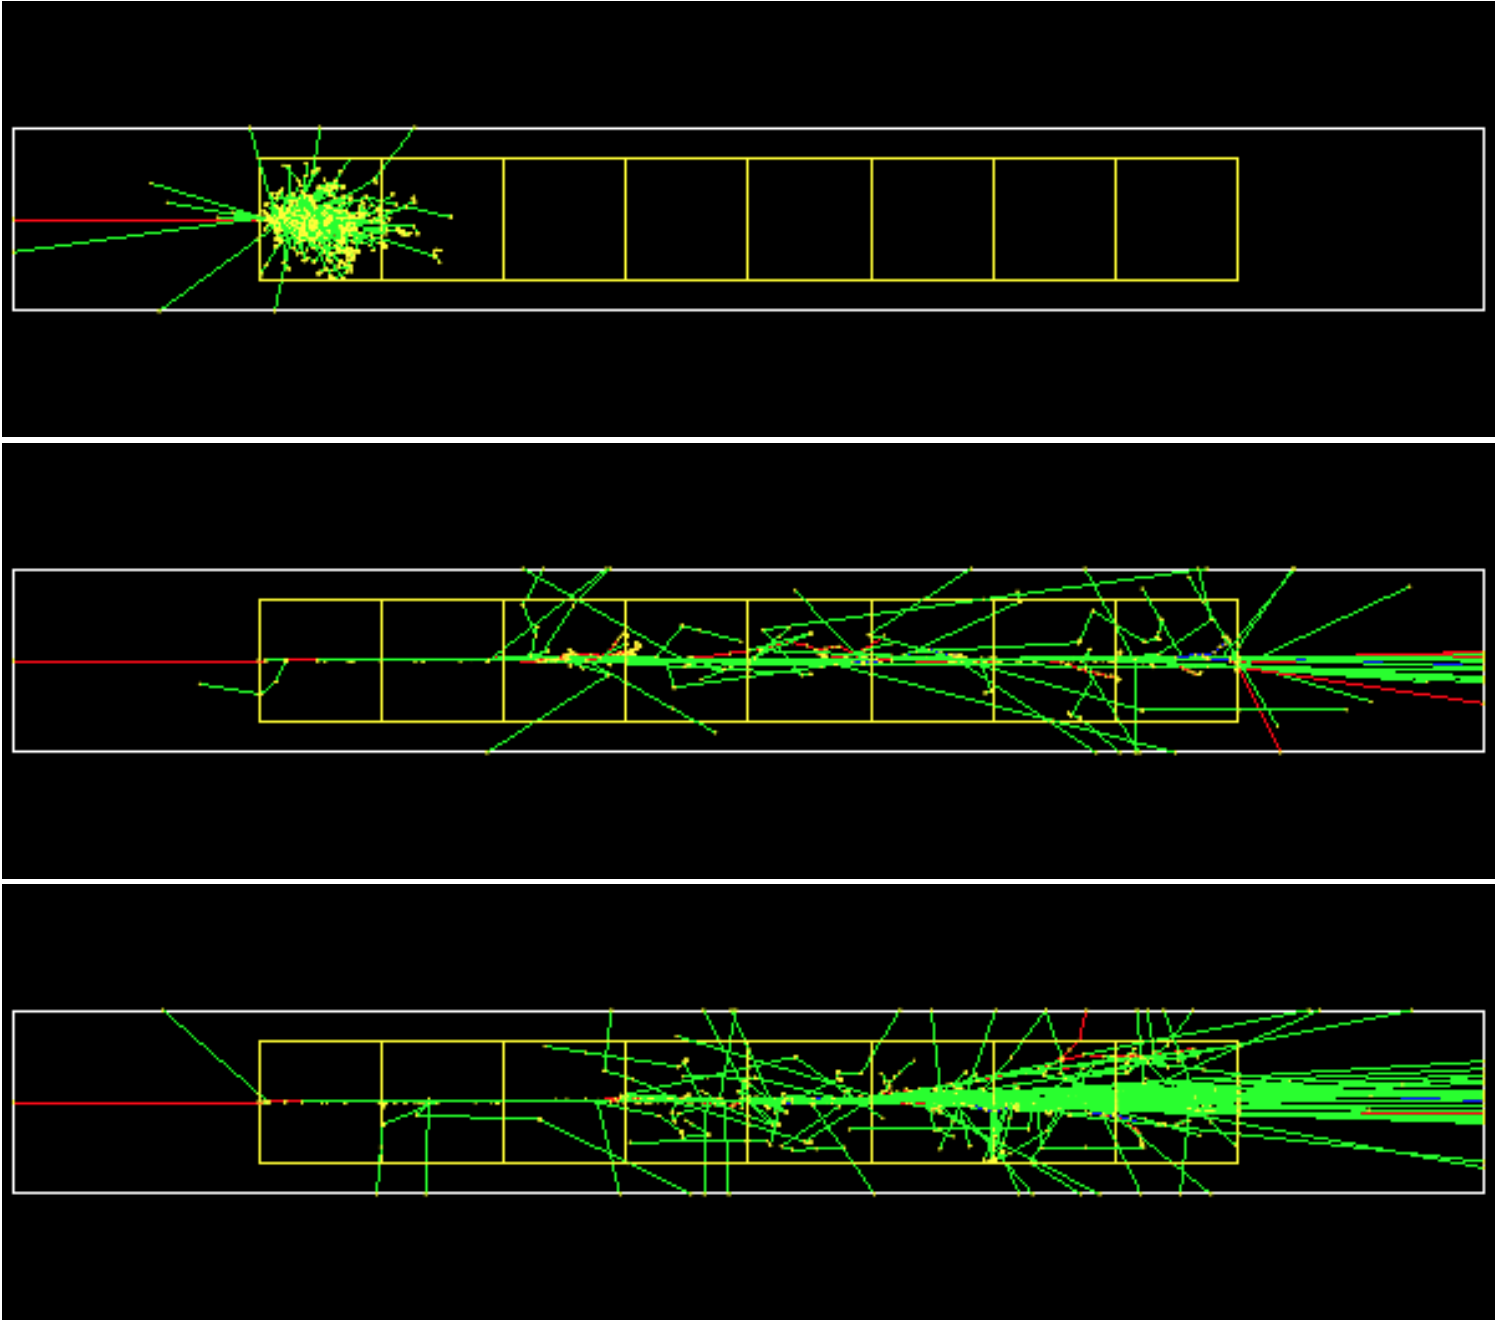
\includegraphics[width=0.44\textwidth]{pics/electron_ed.png}}
  \hfill
  \subfloat[Muon events \label{fig:mu-geo}]
  {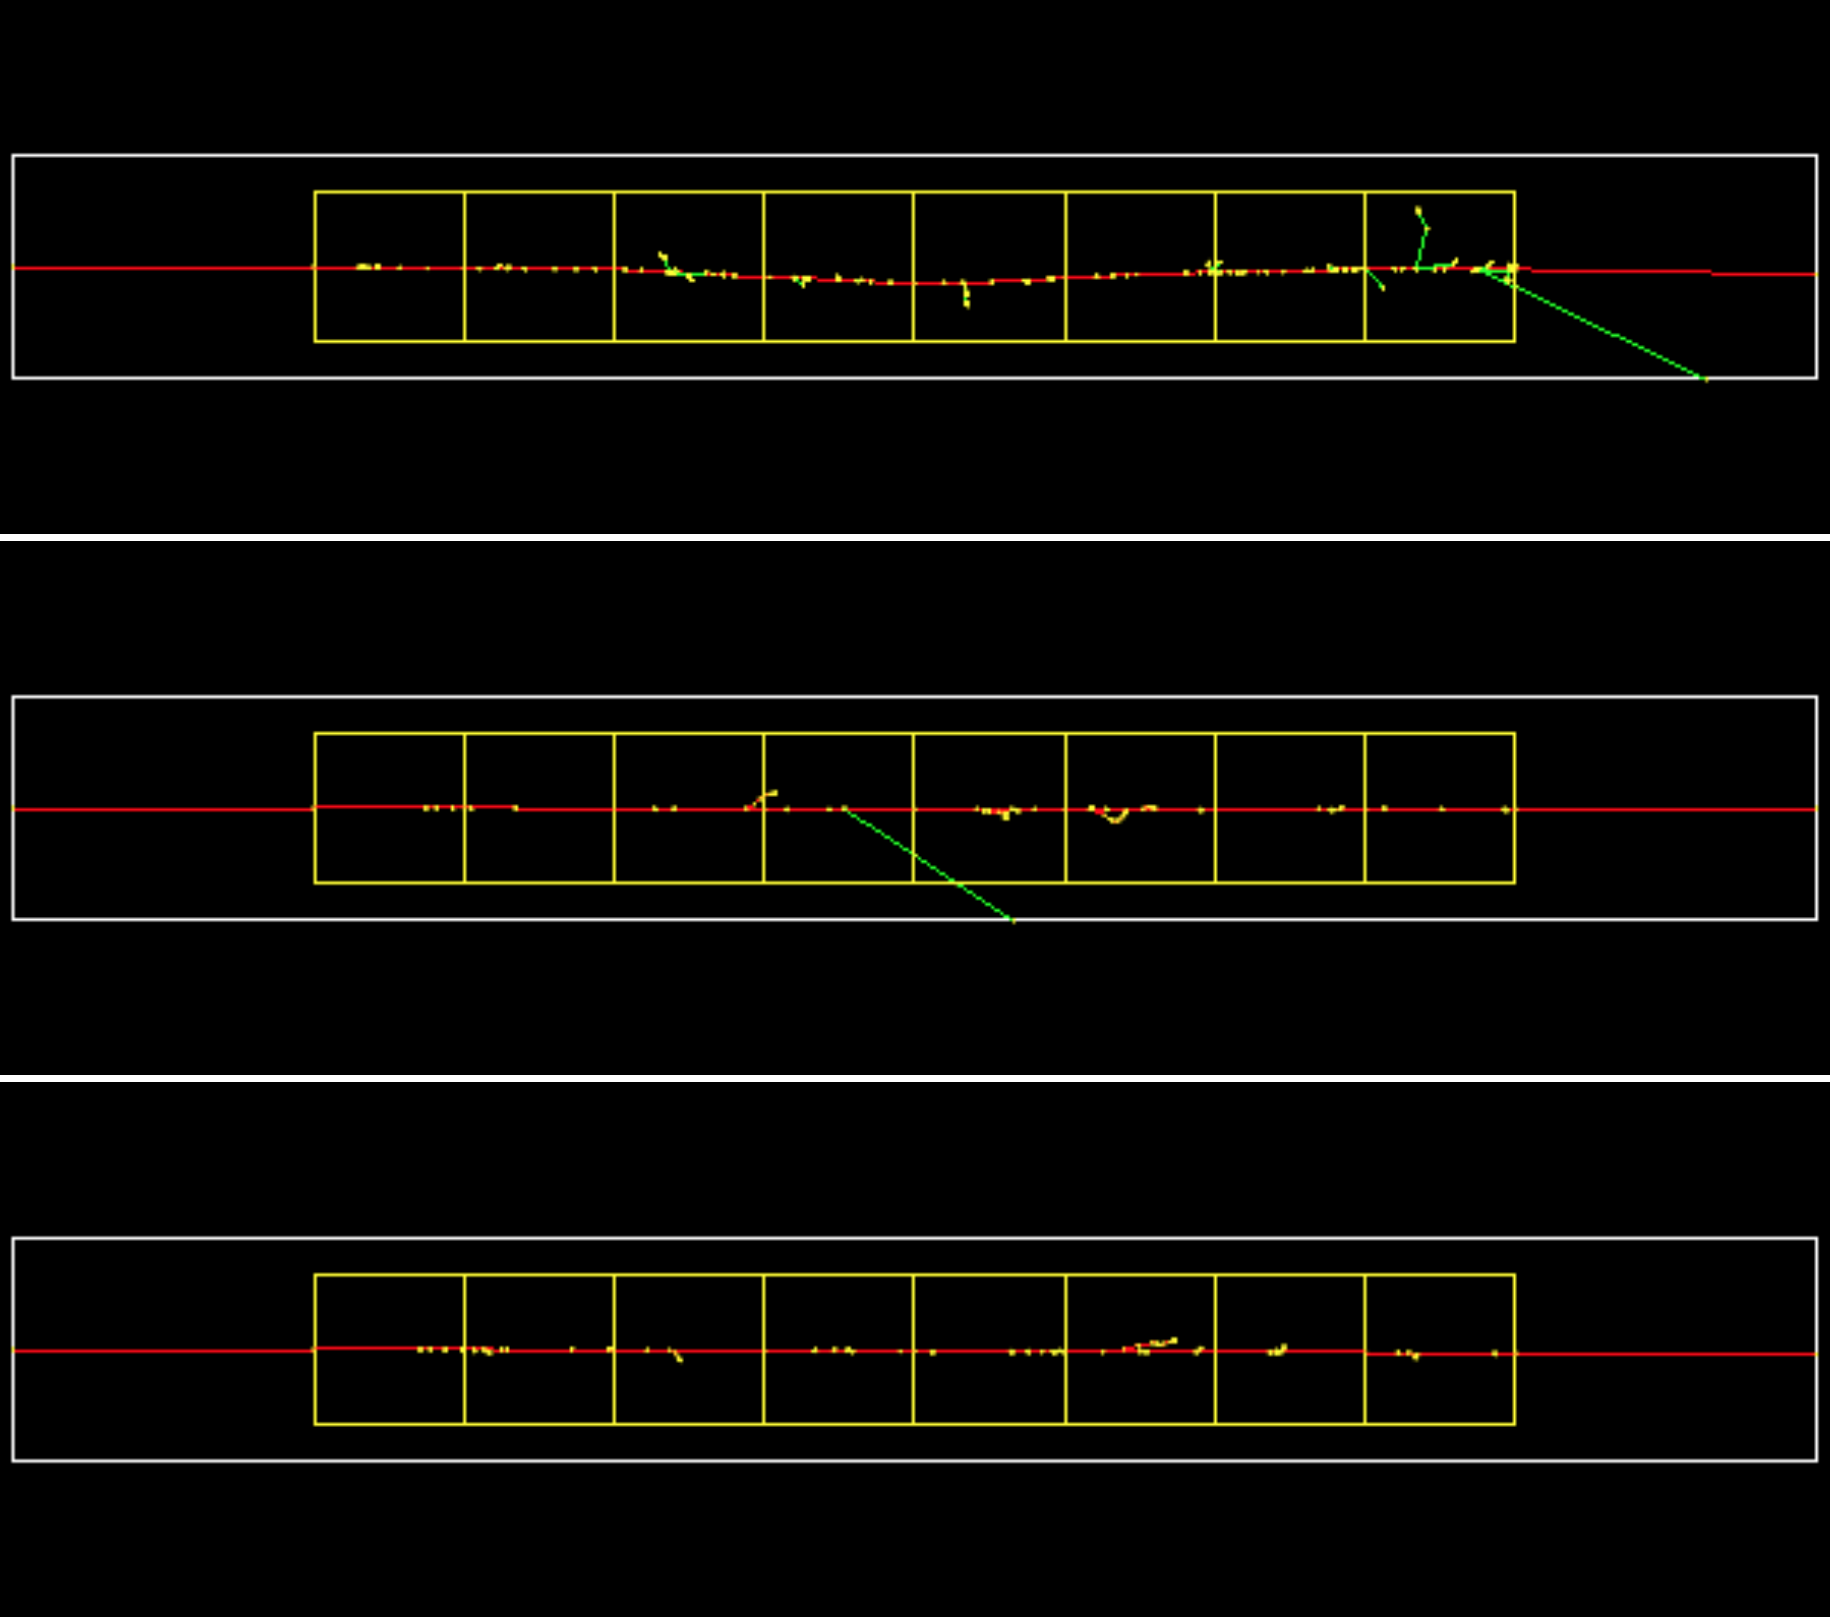
\includegraphics[width=0.44\textwidth]{pics/muon_ed.png}}
  \hfill
  \subfloat[Proton events \label{fig:P-geo}]
  {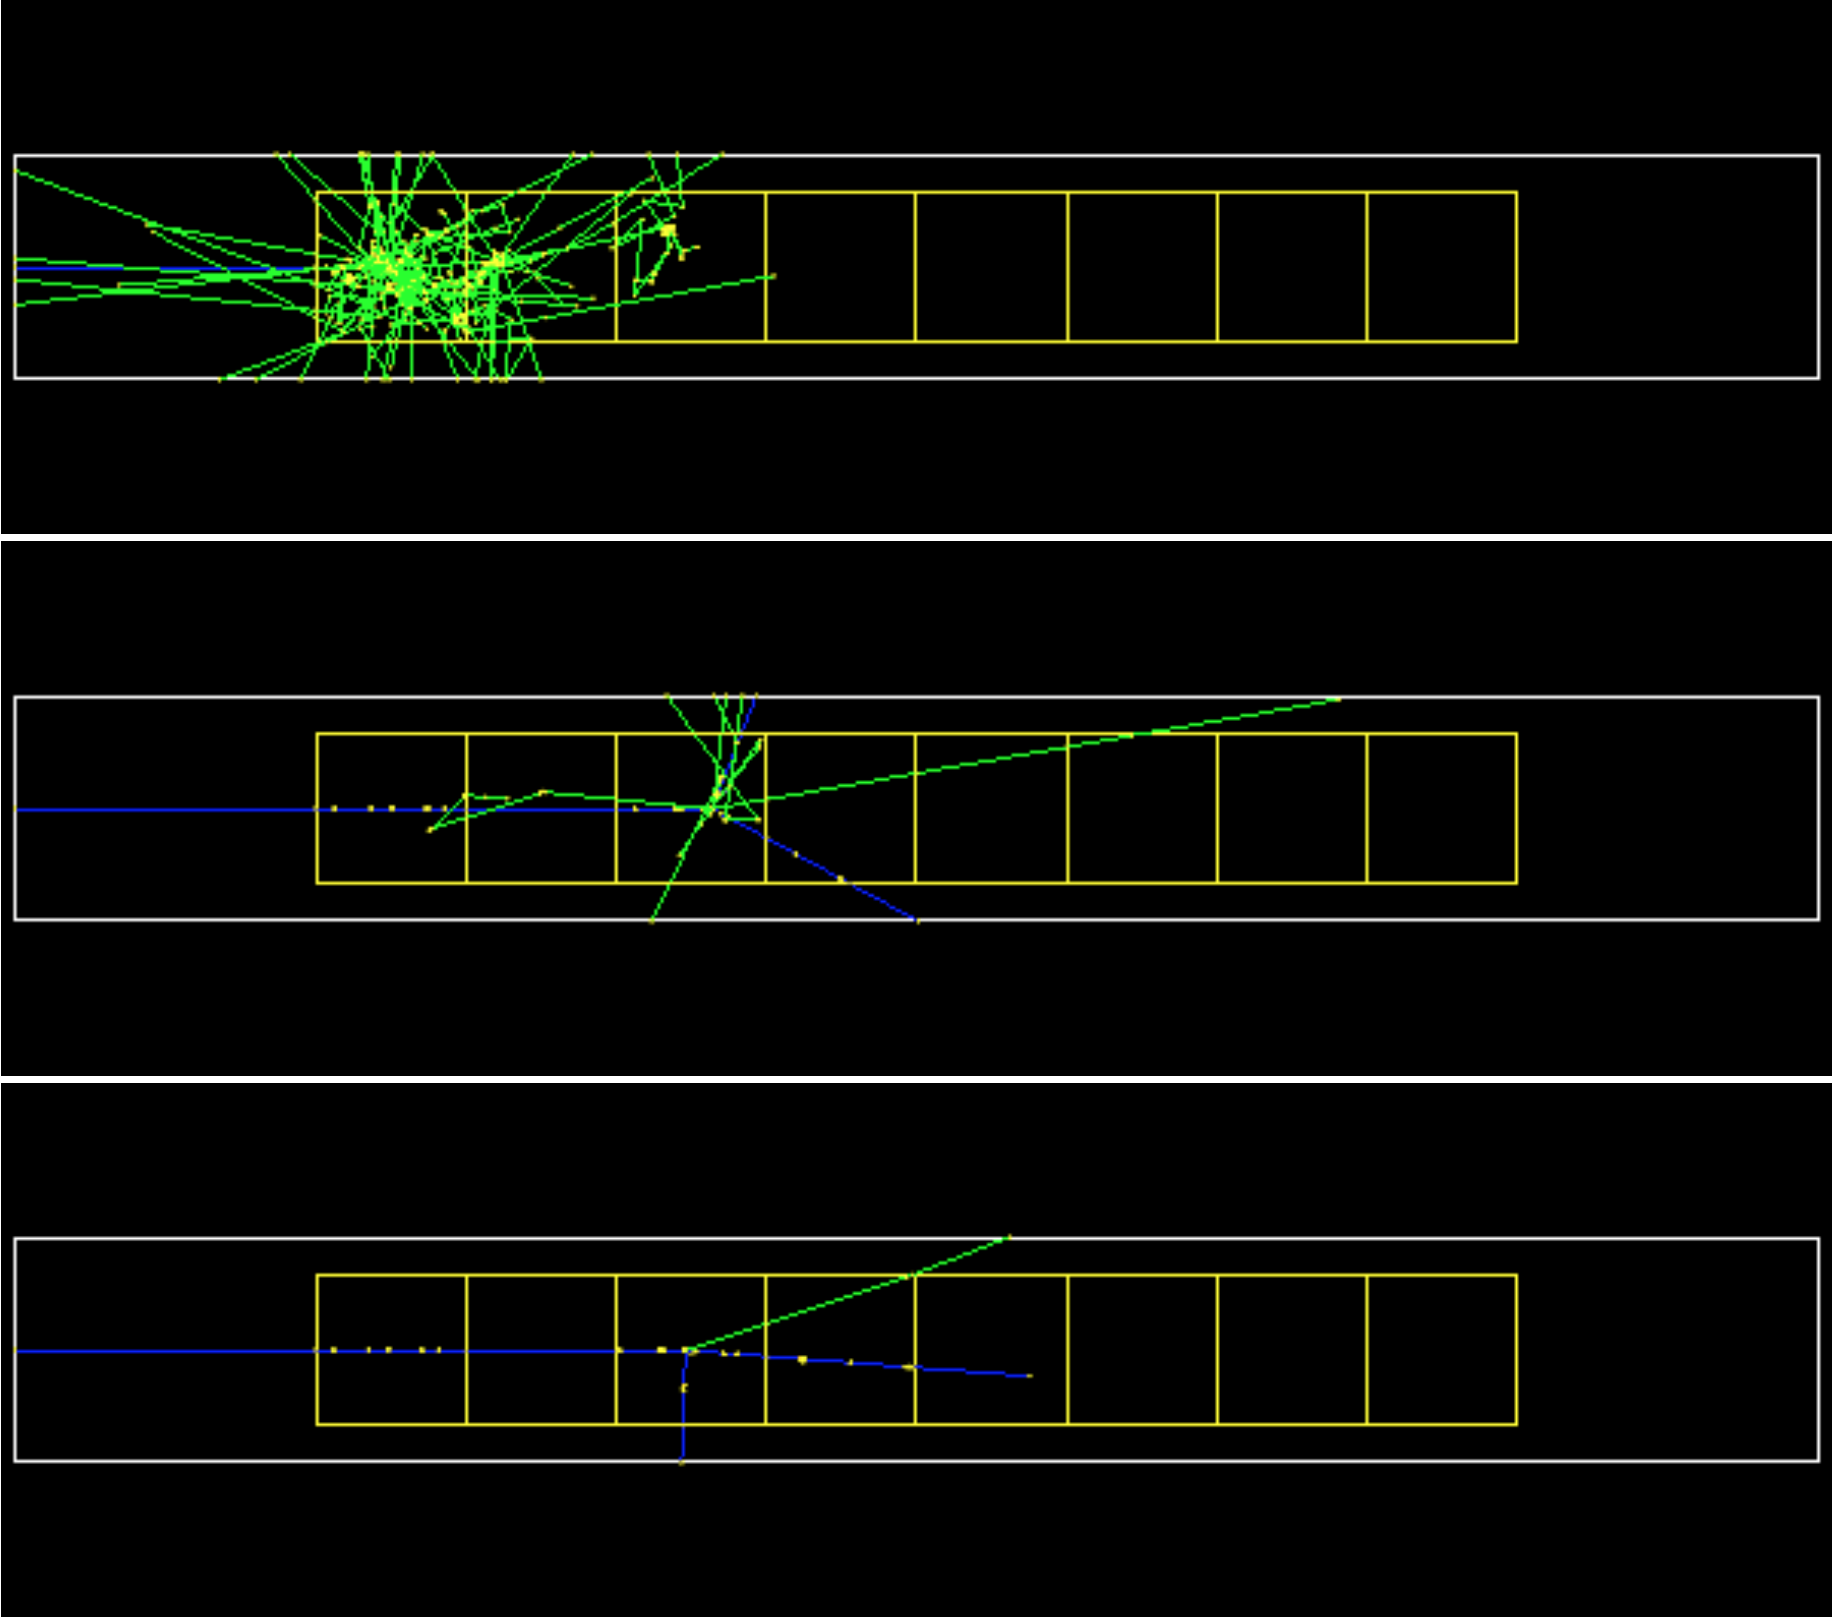
\includegraphics[width=0.44\textwidth]{pics/proton_ed.png}}
  \hfill
  \subfloat[Neutron events \label{fig:N-geo}]
  {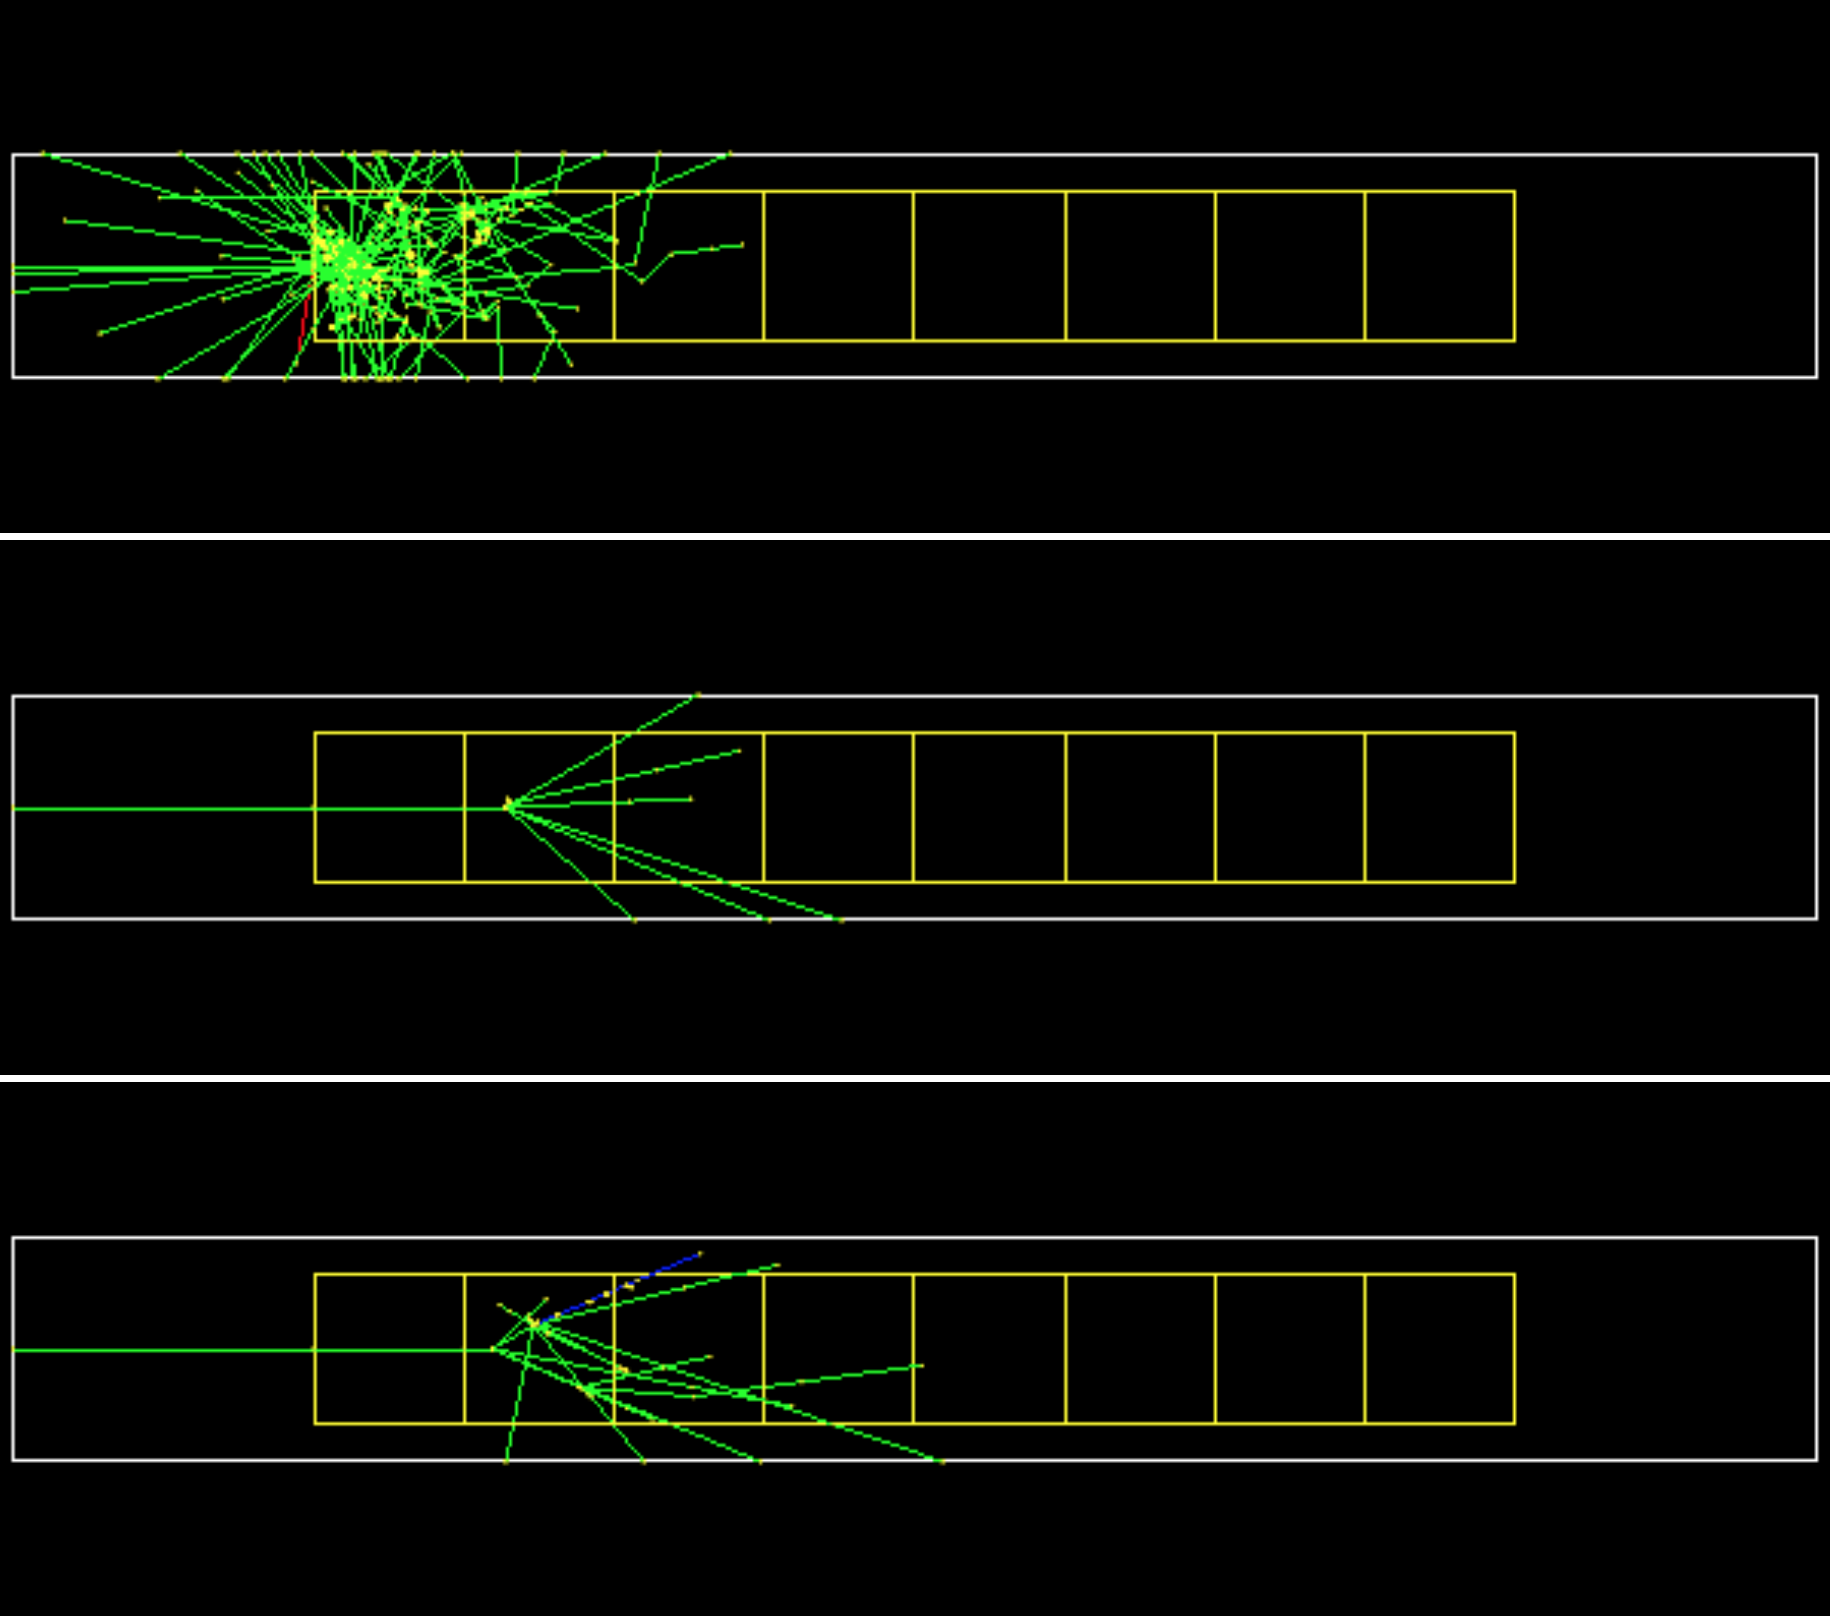
\includegraphics[width=0.44\textwidth]{pics/neutron_ed.png}}
  \caption{The detector geometry with a 2 GeV particle events in three different materials. The top displays corresponds to lead, the middle displays to polypropylene, and the bottom displays to water. Red trajectories indicate negatively charged tracks, green neutral tracks, and blue positively charged tracks.}
  \label{fig:mean and std of nets}
\end{figure*}

\subsection{Quantitative Results}

The deposited energy and average track length per layer plots generally reinforce the impressions gained from viewing the visualizations. The Pb absorbs all four types of particles very rapidly while the polypropylene and water do not halt the particles as fast and behave very similarly to each other. This is likely due to both of them containing large numbers of H nuclei, bound to either O or C, for the incoming particles to interact with.

One interesting artifact in the plots can be seen in the average track length per layer plot for the neutron runs. For both polypropylene and water the first bin for 0 track length has an enormous excess of events compared to the rest of the plot. Due to time constraints we were unable to determine the cause of this excess in detail, but due to the picture presented by the deposited energy plots and visualizations it is not likely that these neutrons are really being completely stopped by the polypropylene and water. The spike may be an artifact of the normalization procedure run on this plot. 

\begin{figure*}
  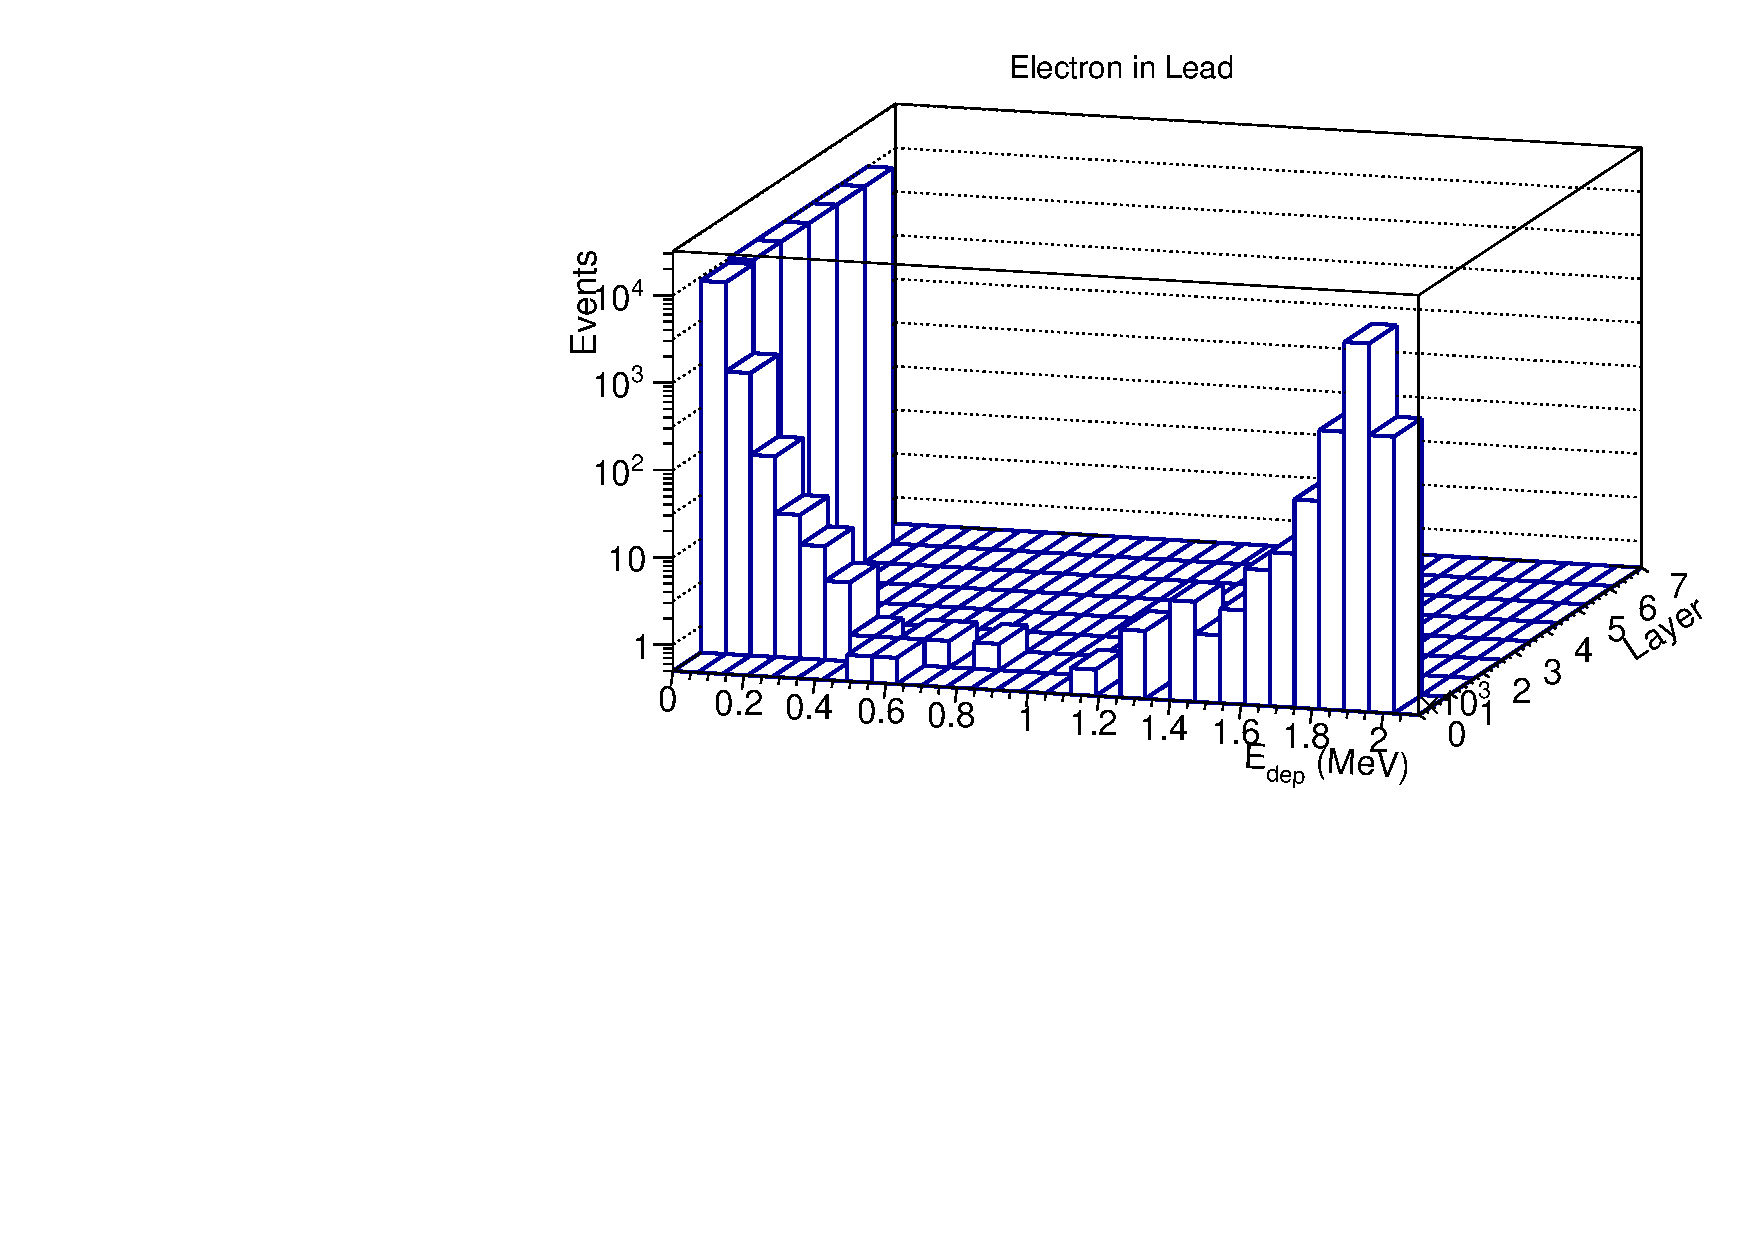
\includegraphics[width=.45\textwidth]{plots/electron_pb_edep.pdf}
  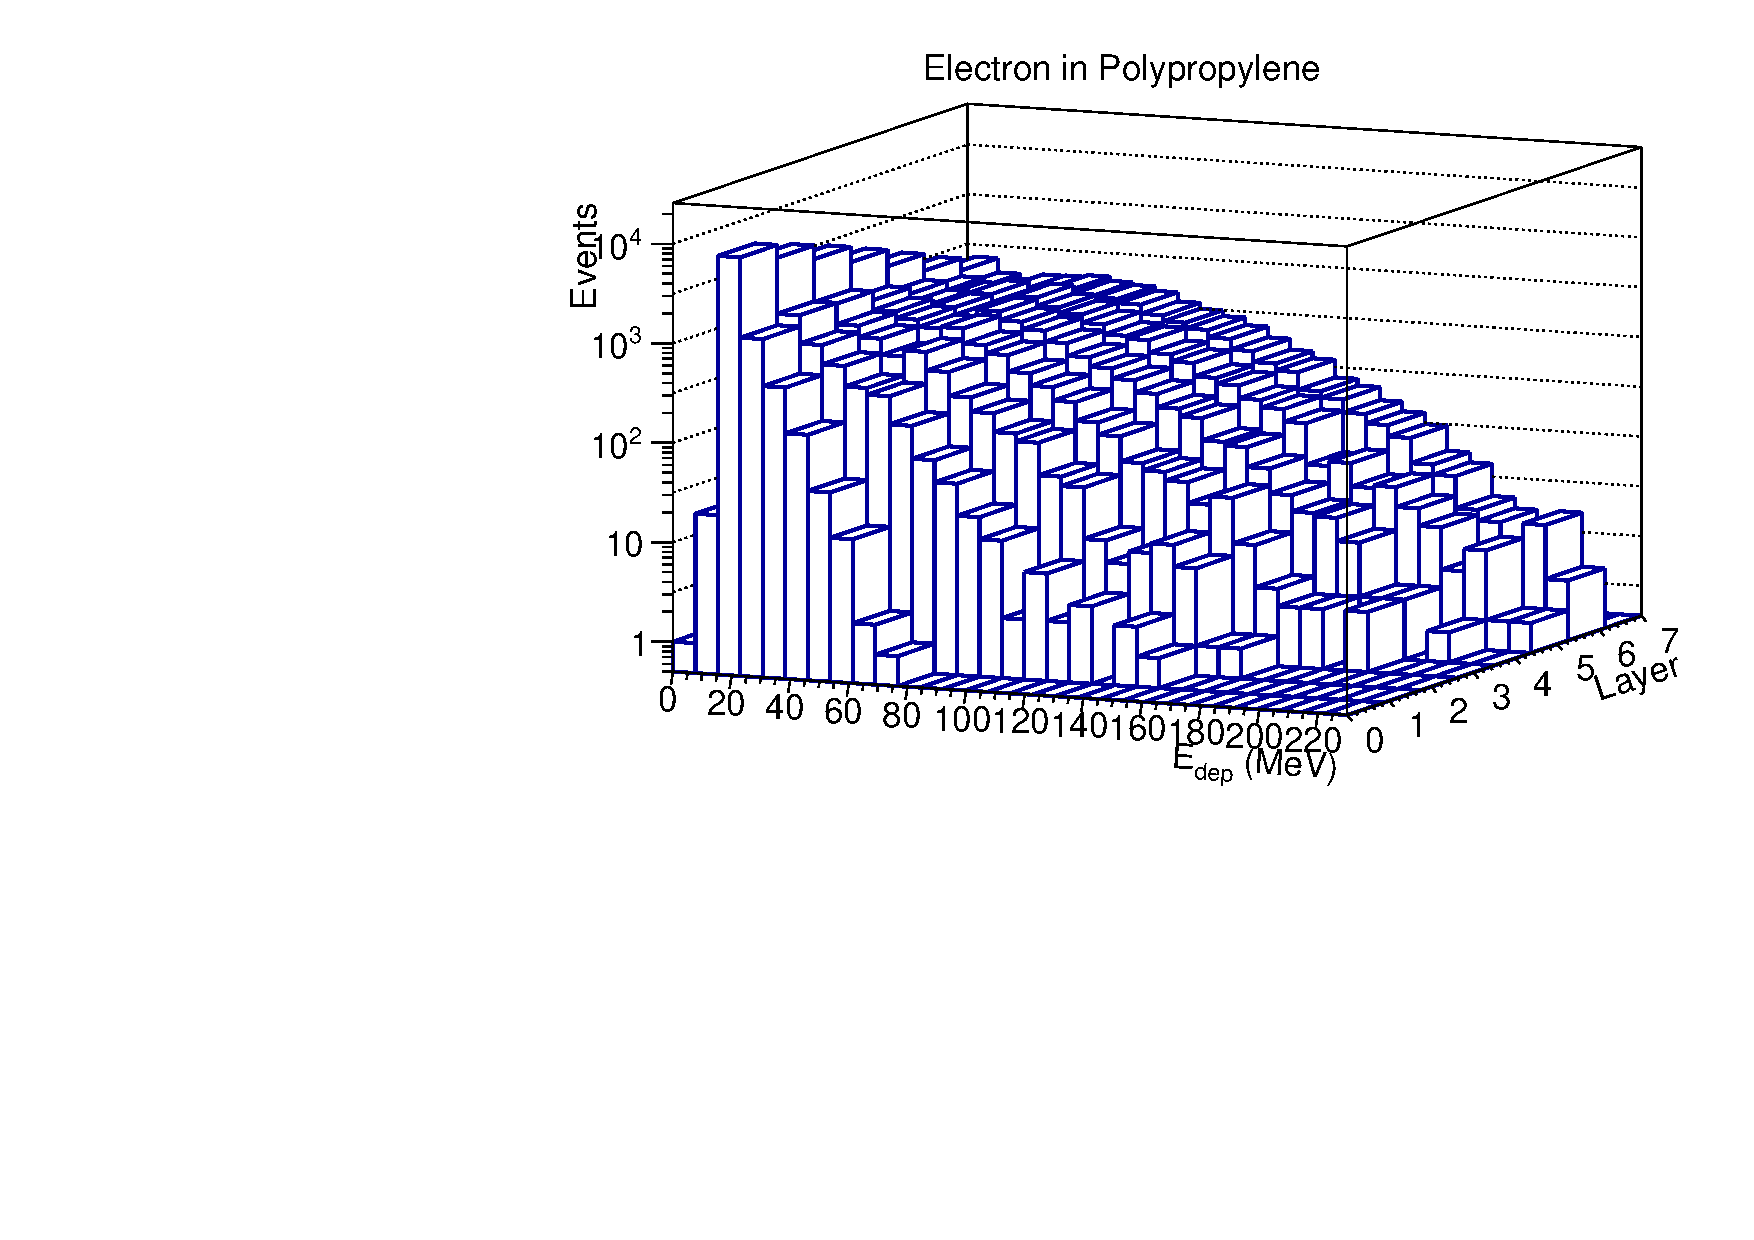
\includegraphics[width=.45\textwidth]{plots/electron_pp_edep.pdf}
  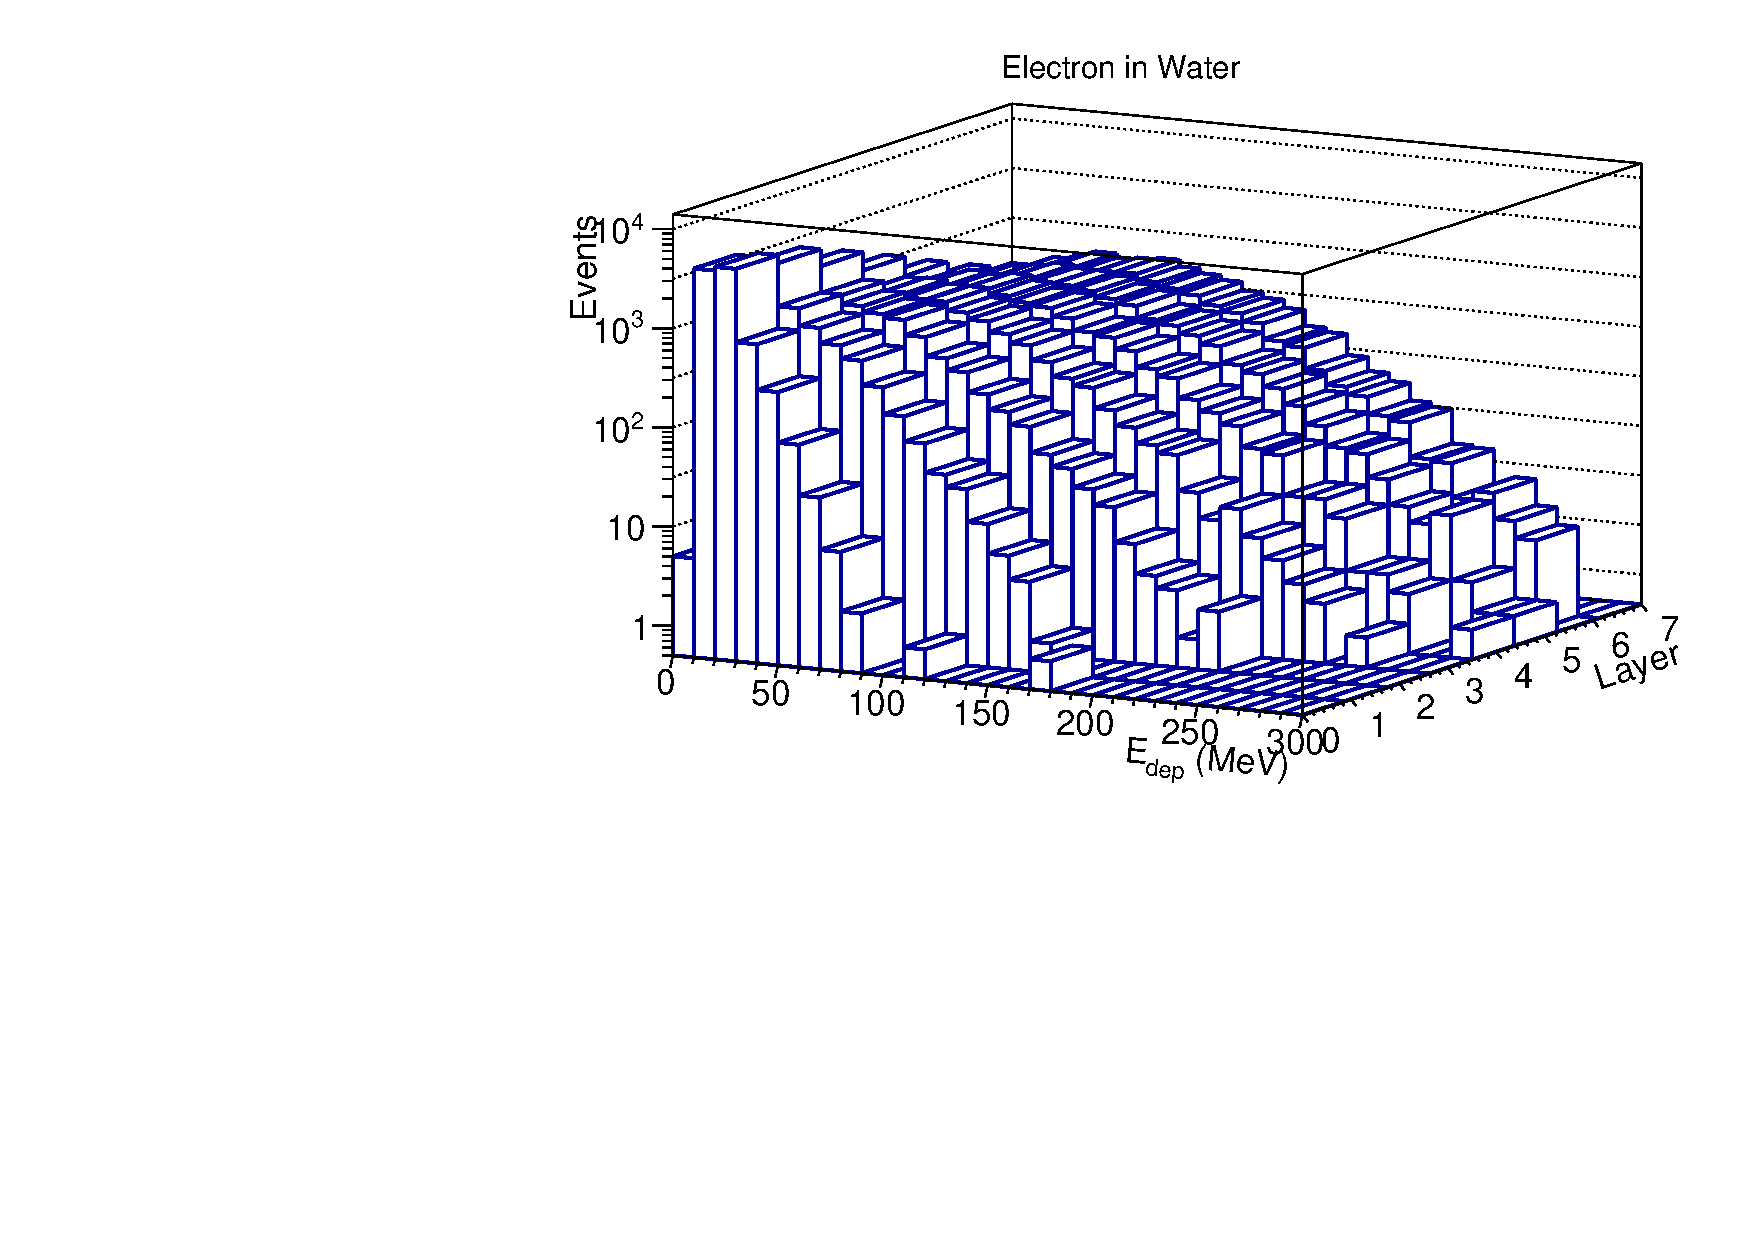
\includegraphics[width=.45\textwidth]{plots/electron_h2o_edep.pdf}
  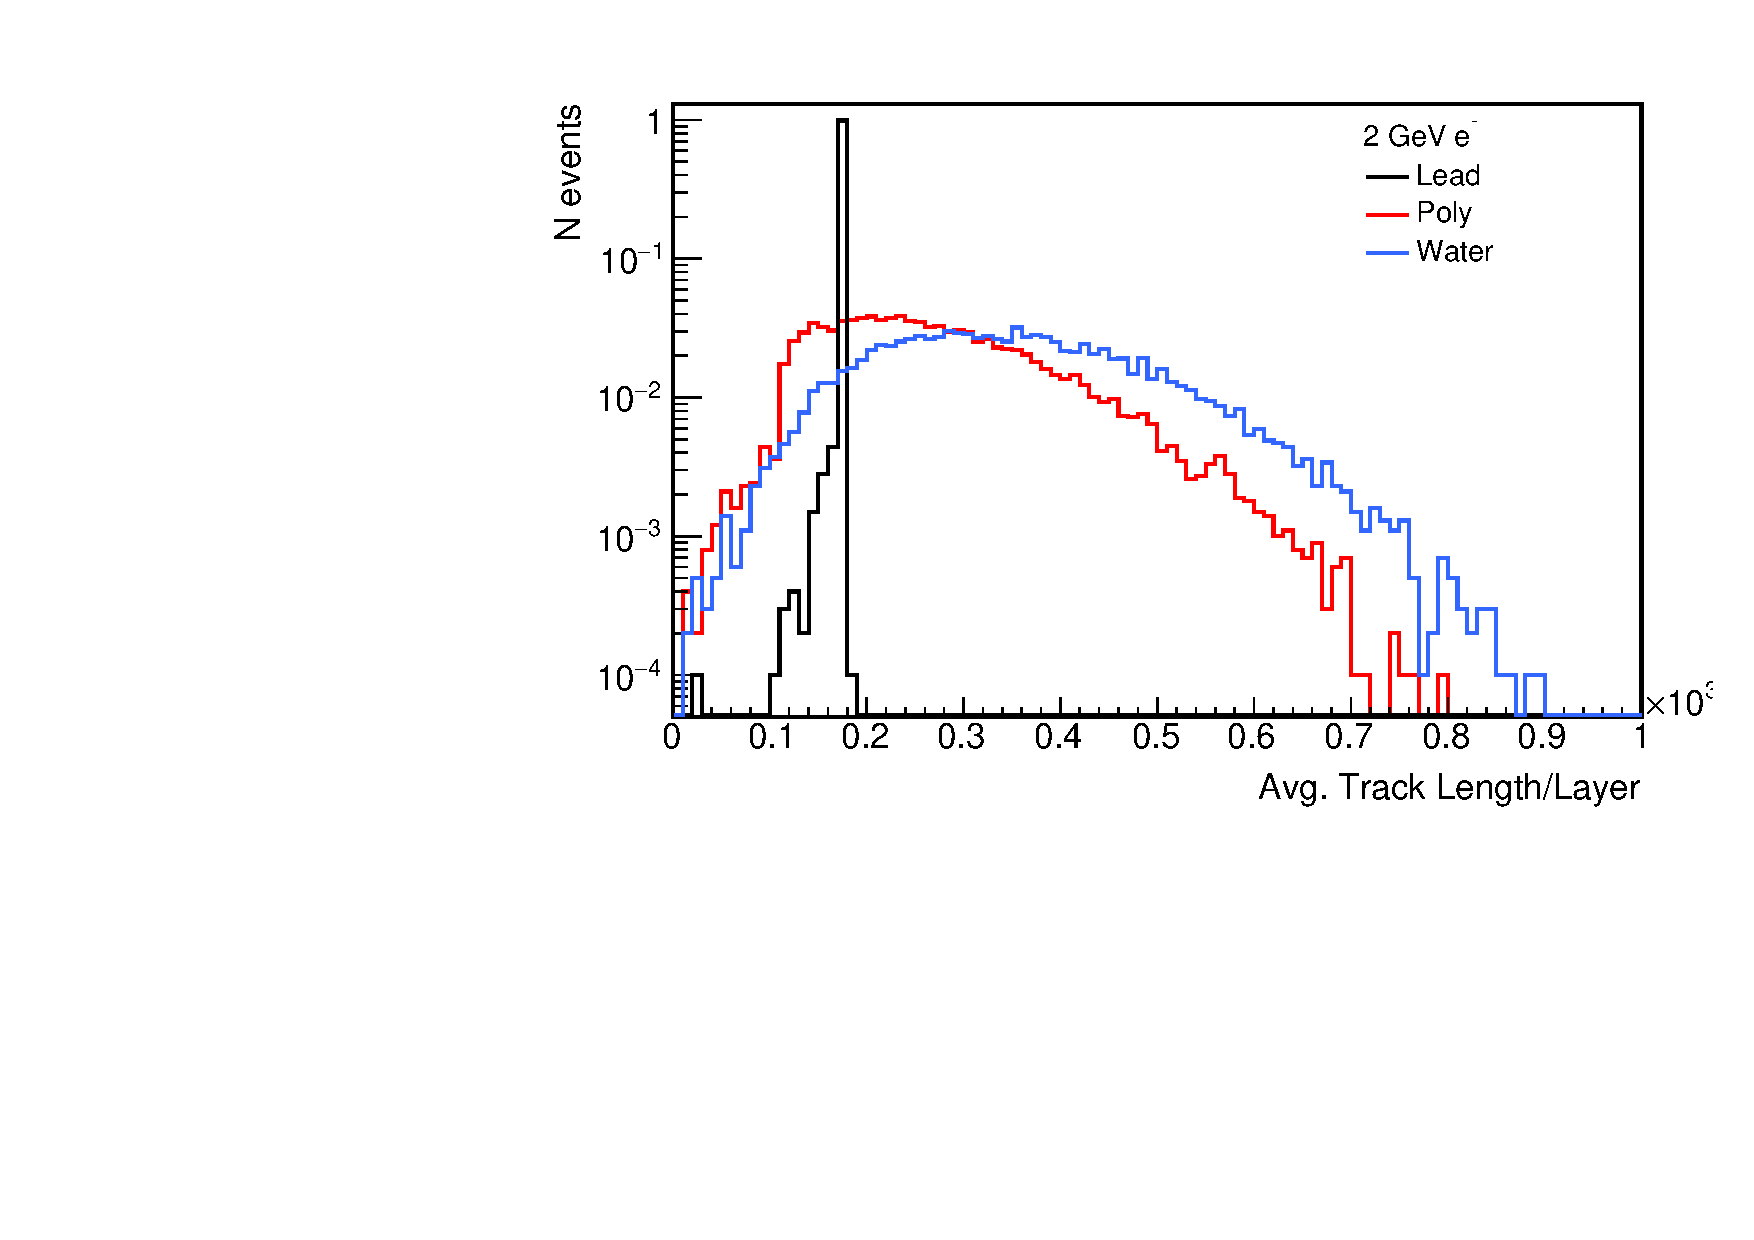
\includegraphics[width=.45\textwidth]{plots/TL_electron.pdf}
  \caption{Electron Plots, Pb $E_{\text{dep}}$ plot effectively has units of GeV not MeV, the $10^3$ is obscured.}
  \label{fig:e-quant}
\end{figure*}

\begin{figure*}
  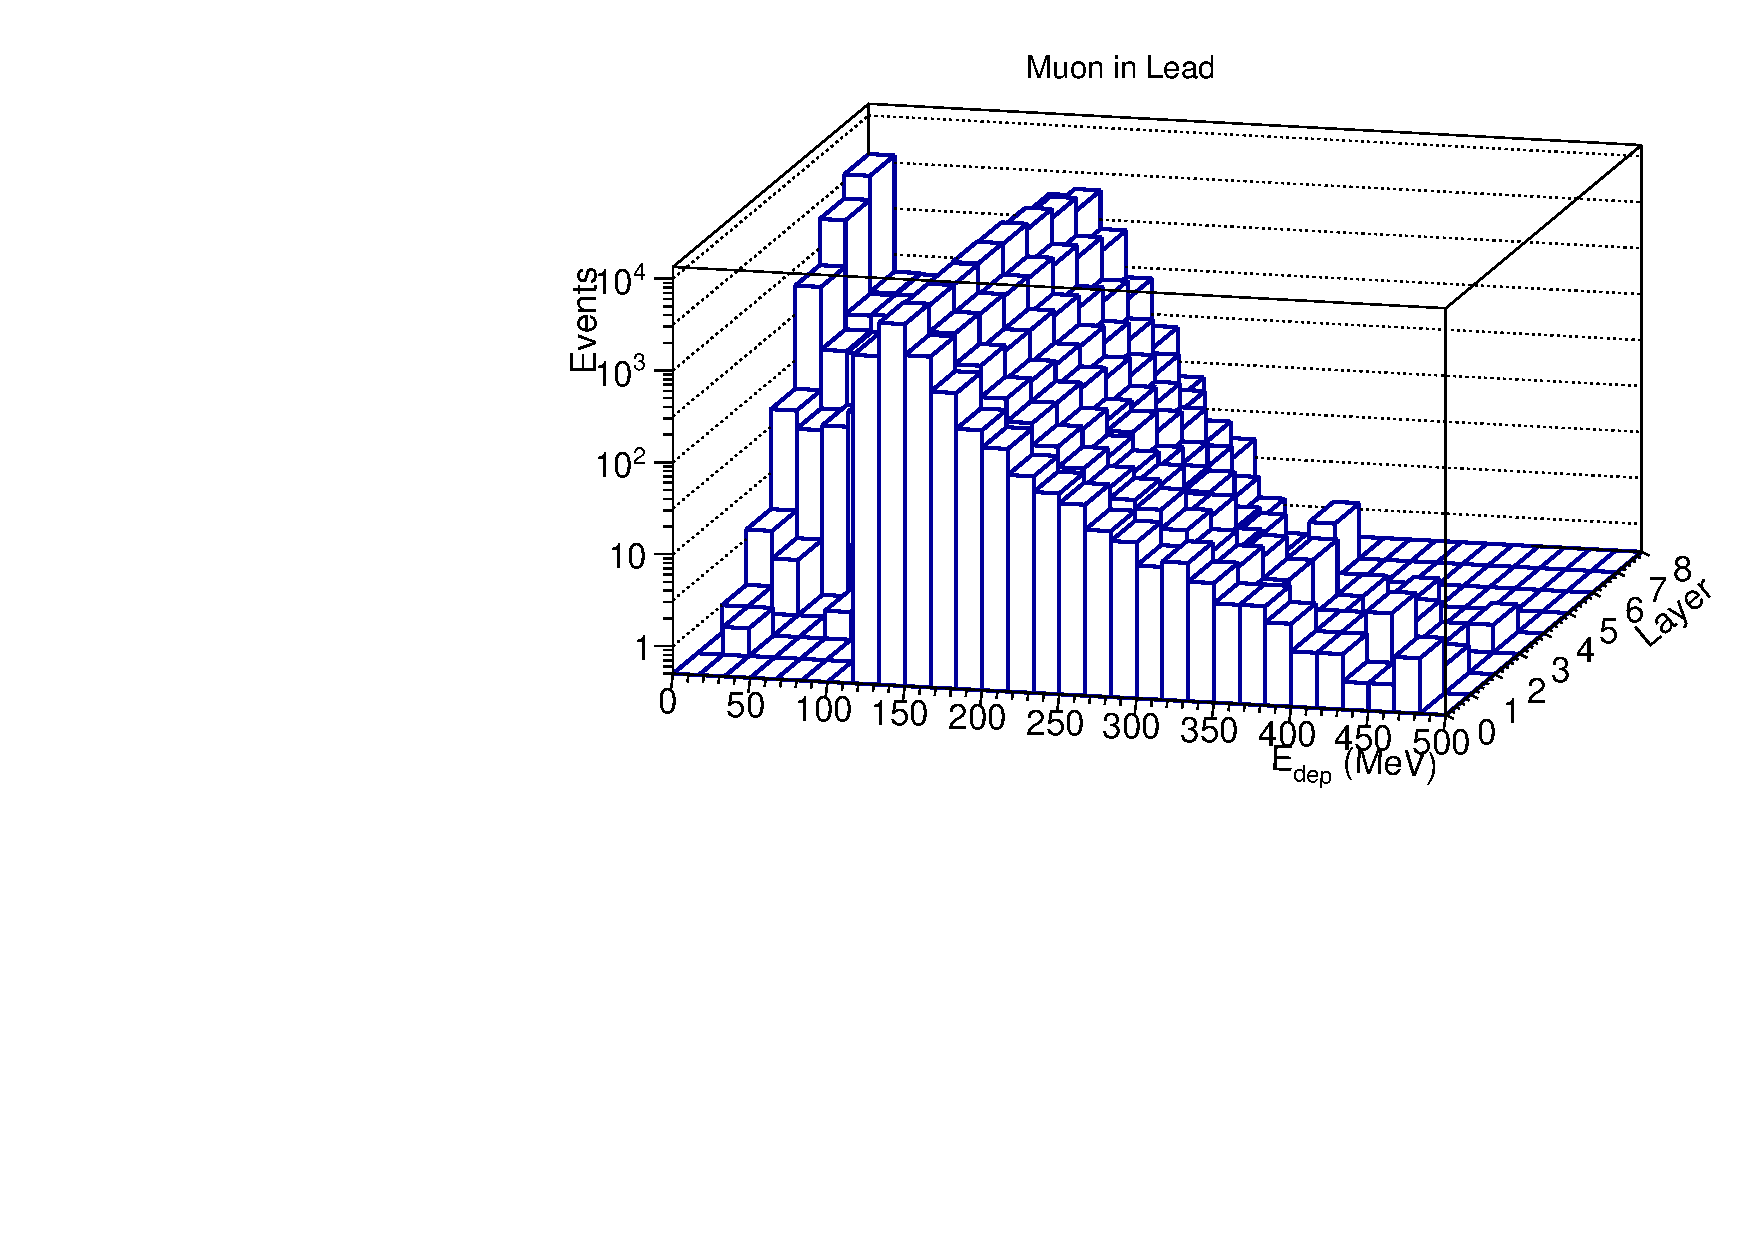
\includegraphics[width=.45\textwidth]{plots/muon_pb_edep.pdf}
  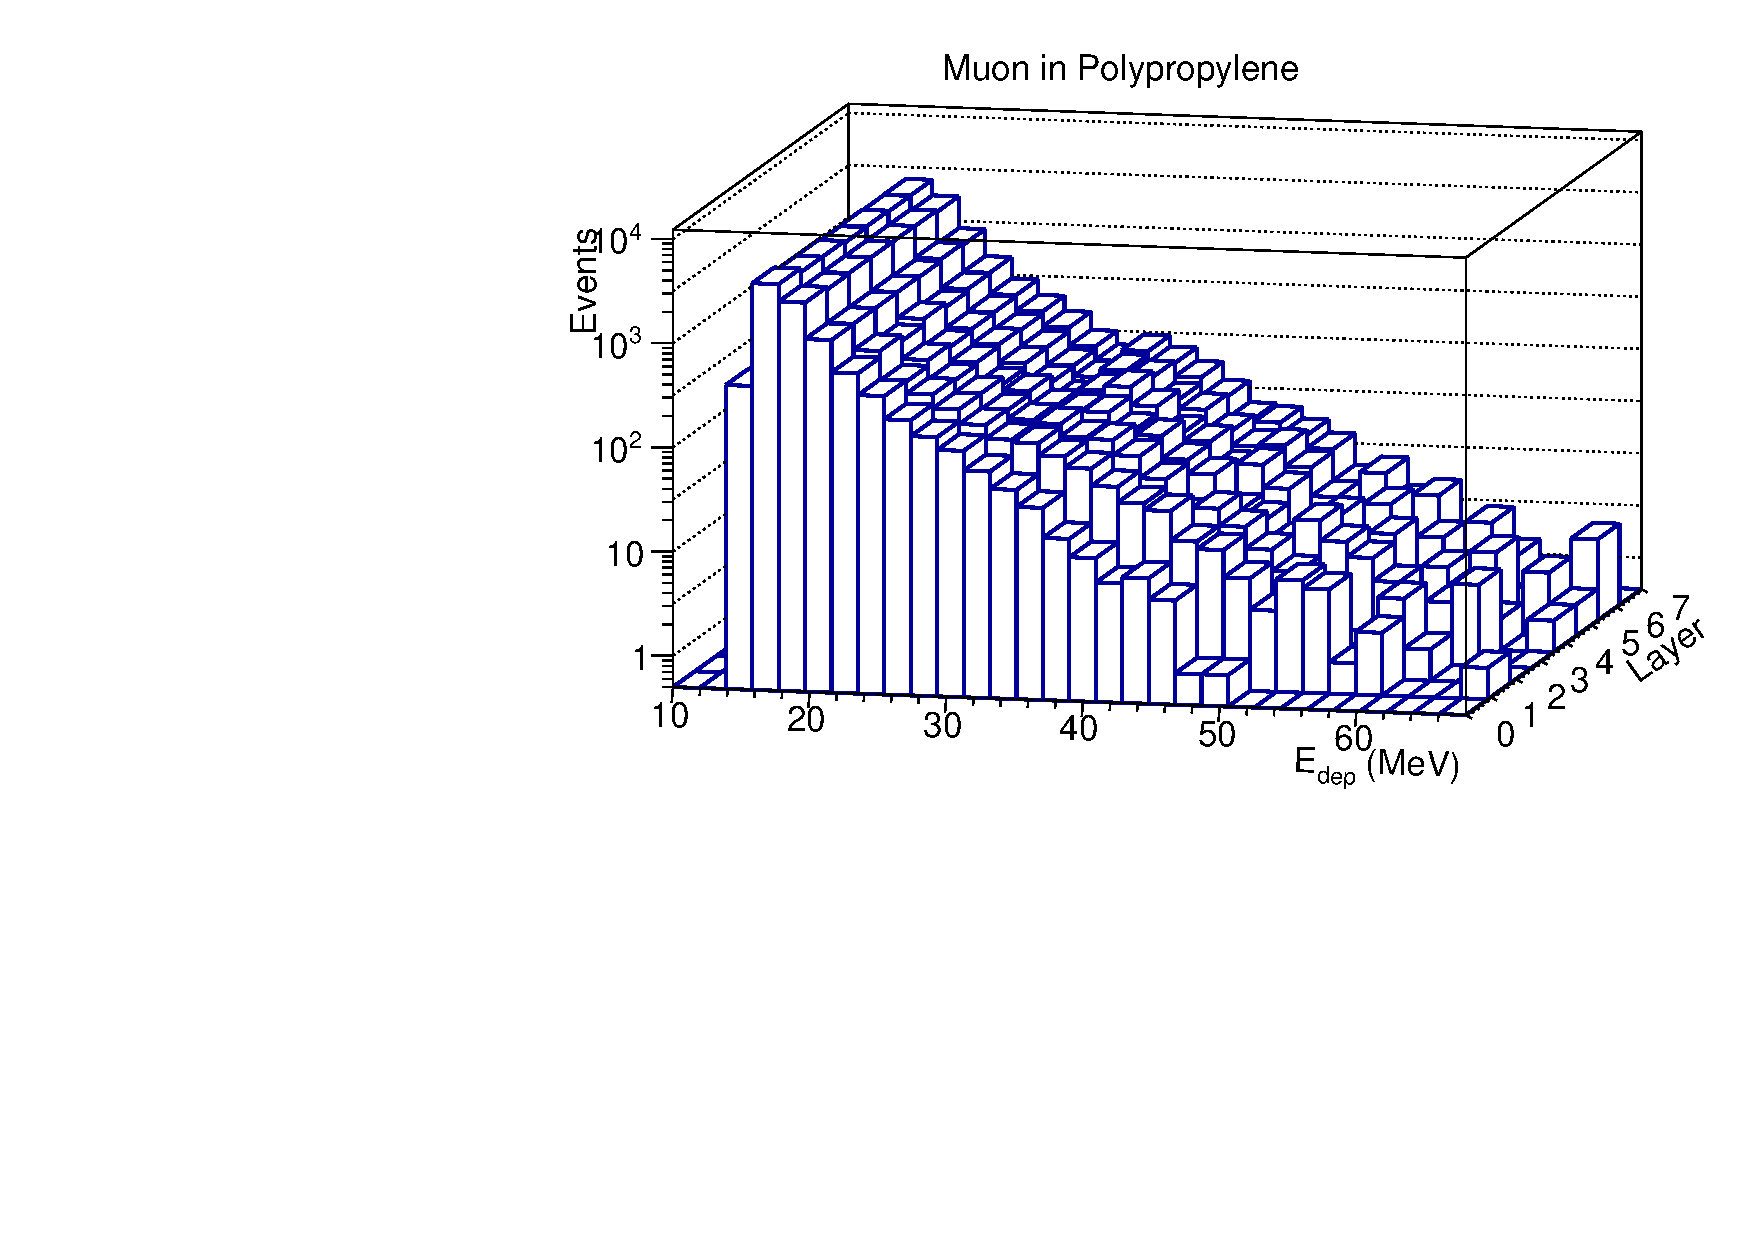
\includegraphics[width=.45\textwidth]{plots/muon_pp_edep.pdf}
  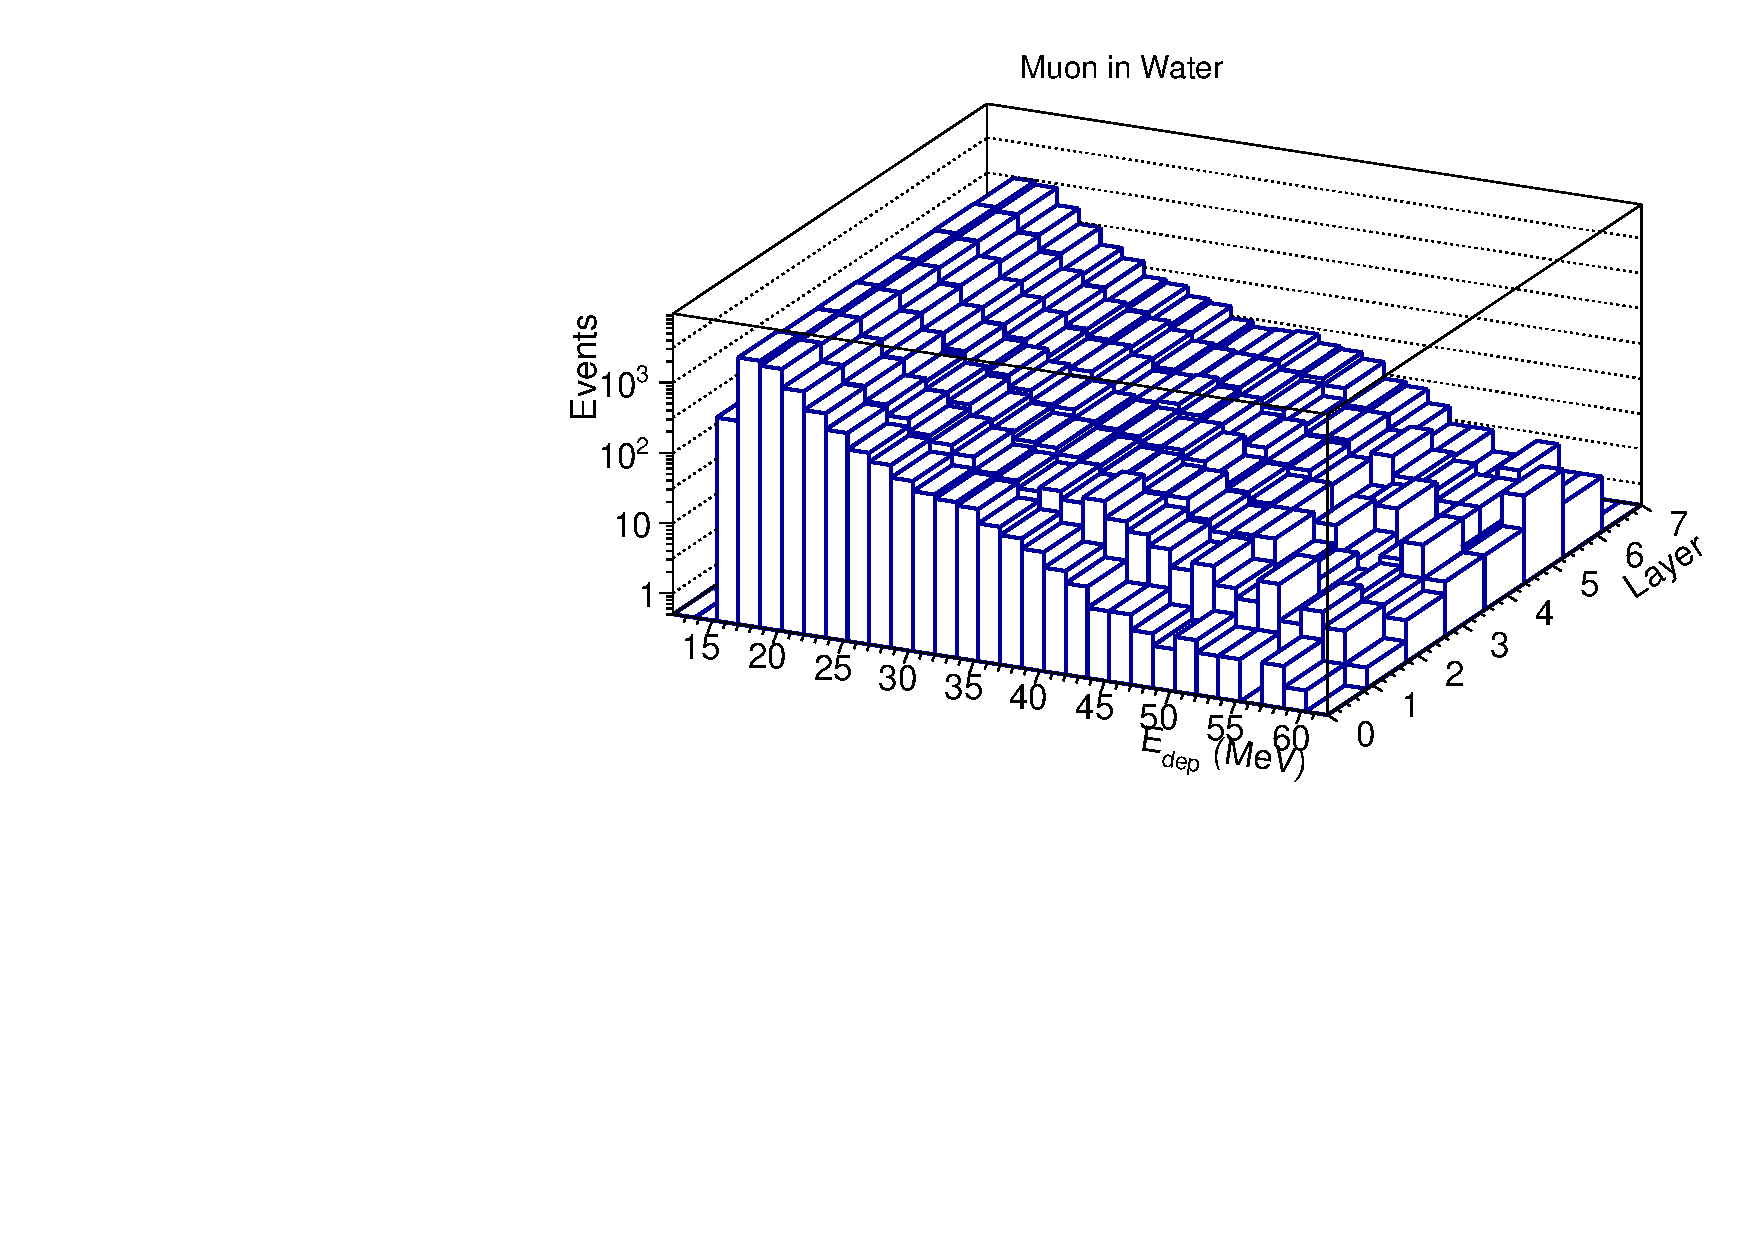
\includegraphics[width=.45\textwidth]{plots/muon_h2o_edep.pdf}
  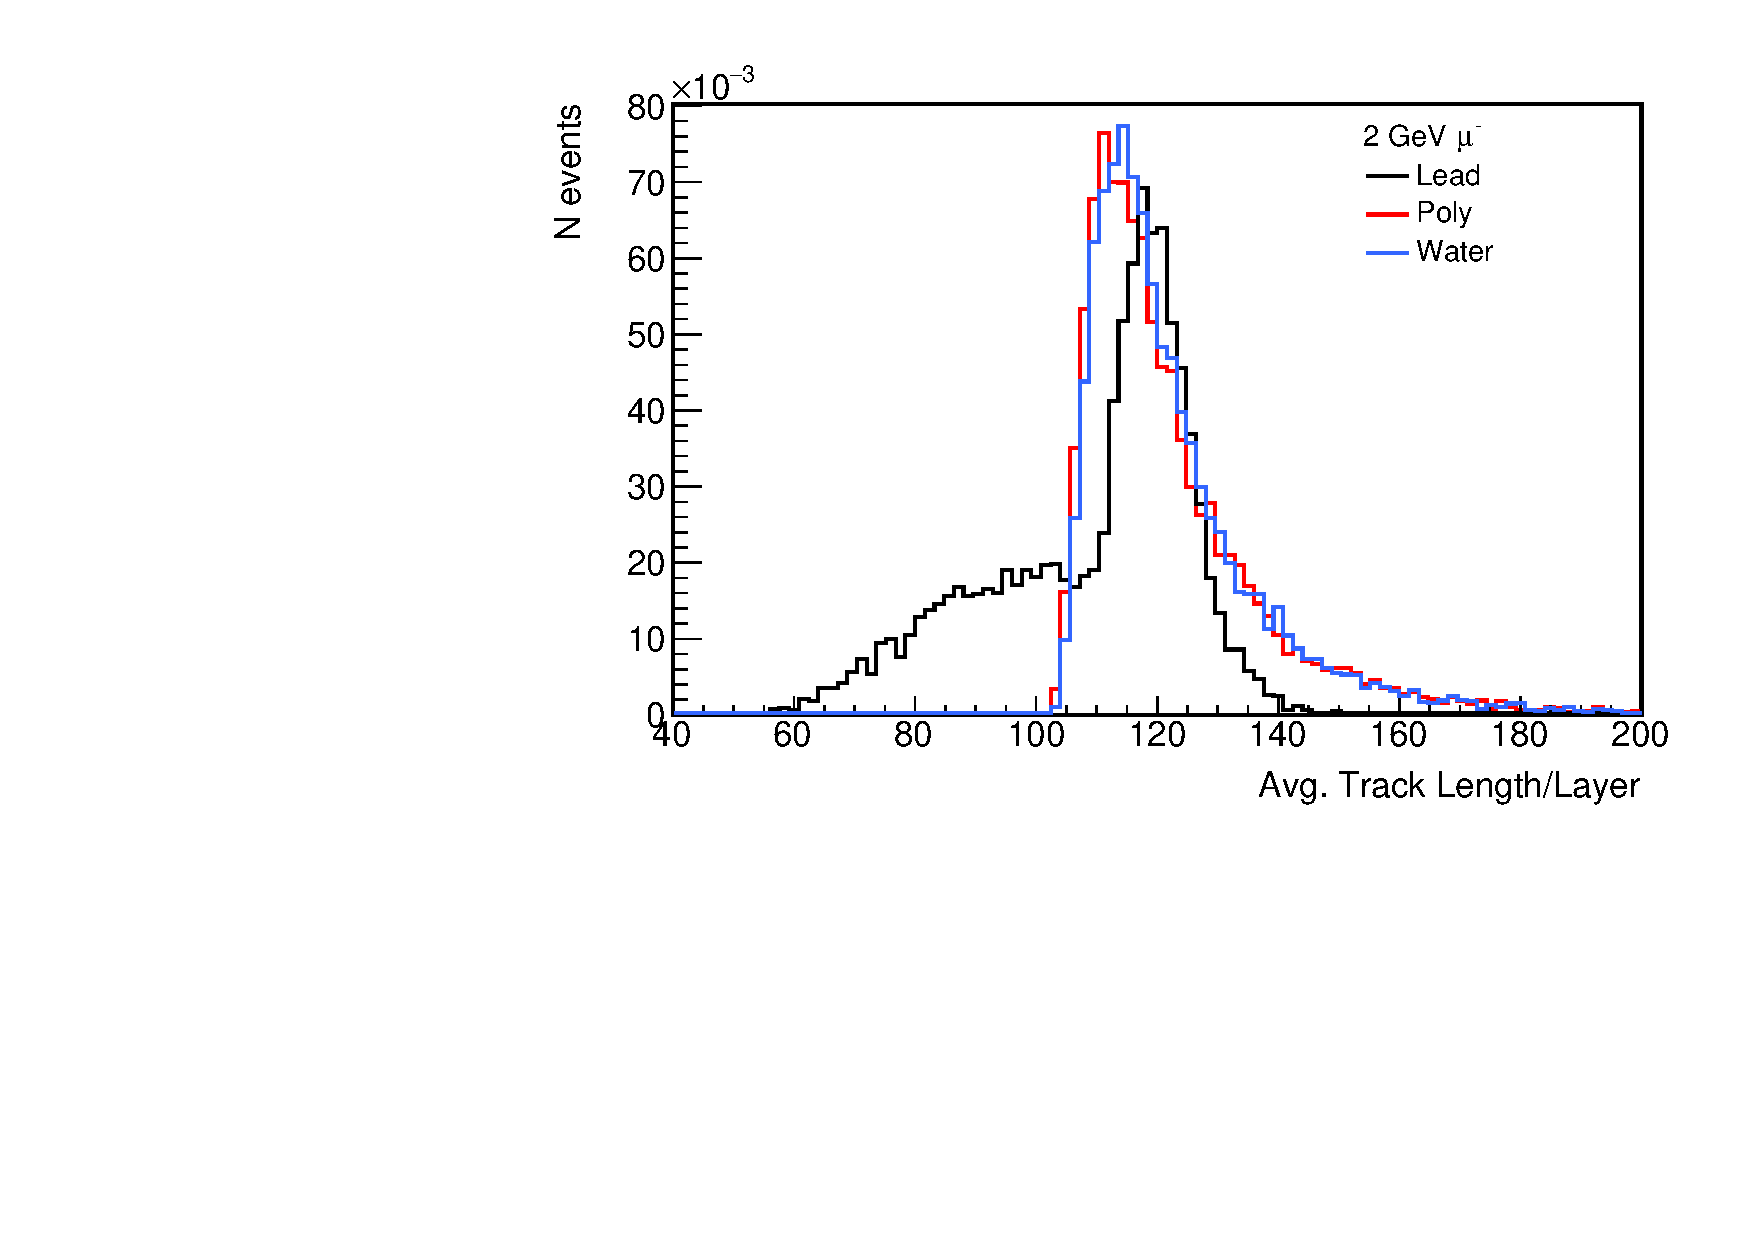
\includegraphics[width=.45\textwidth]{plots/TL_muon.pdf}
  \caption{Muon Plots.}
  \label{fig:mu-quant}
\end{figure*}
\begin{figure*}
  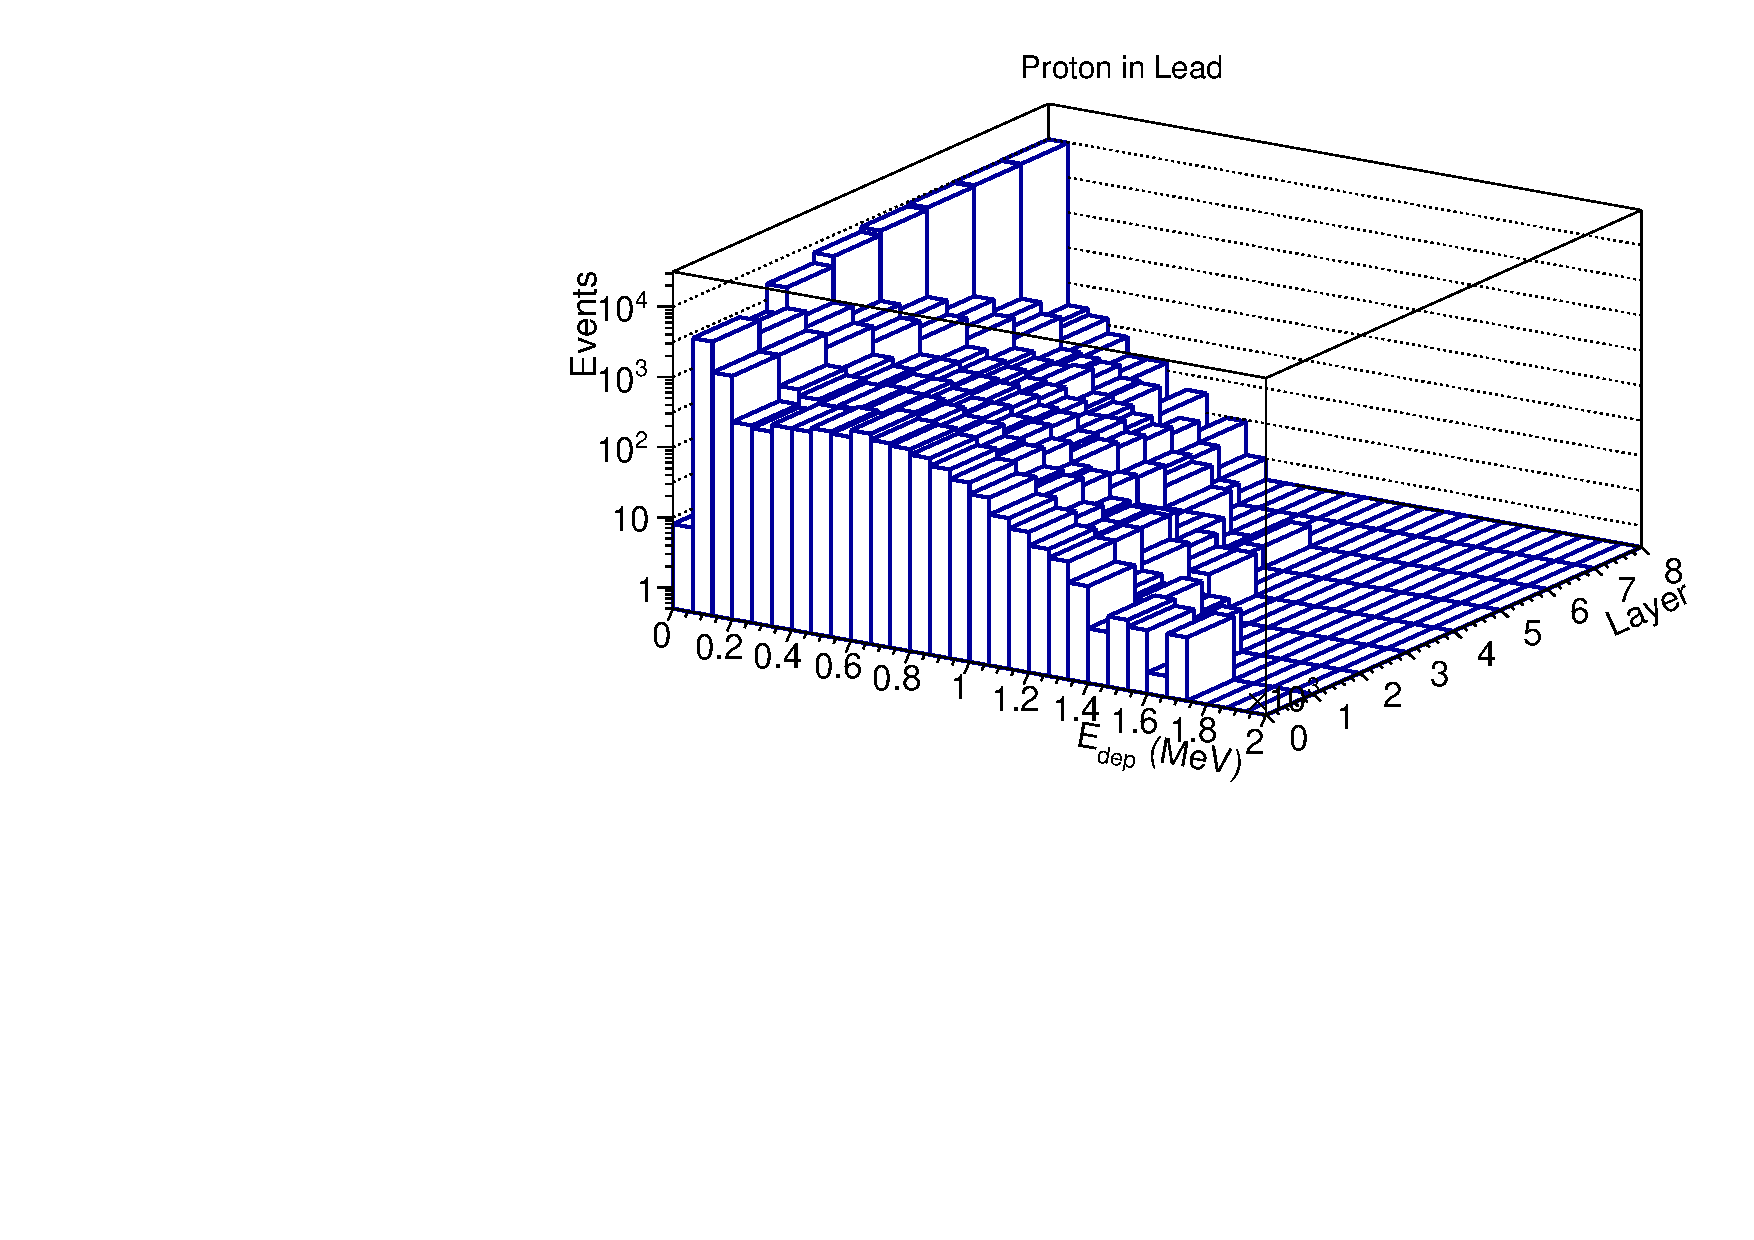
\includegraphics[width=.45\textwidth]{plots/P_pb_edep.pdf}
  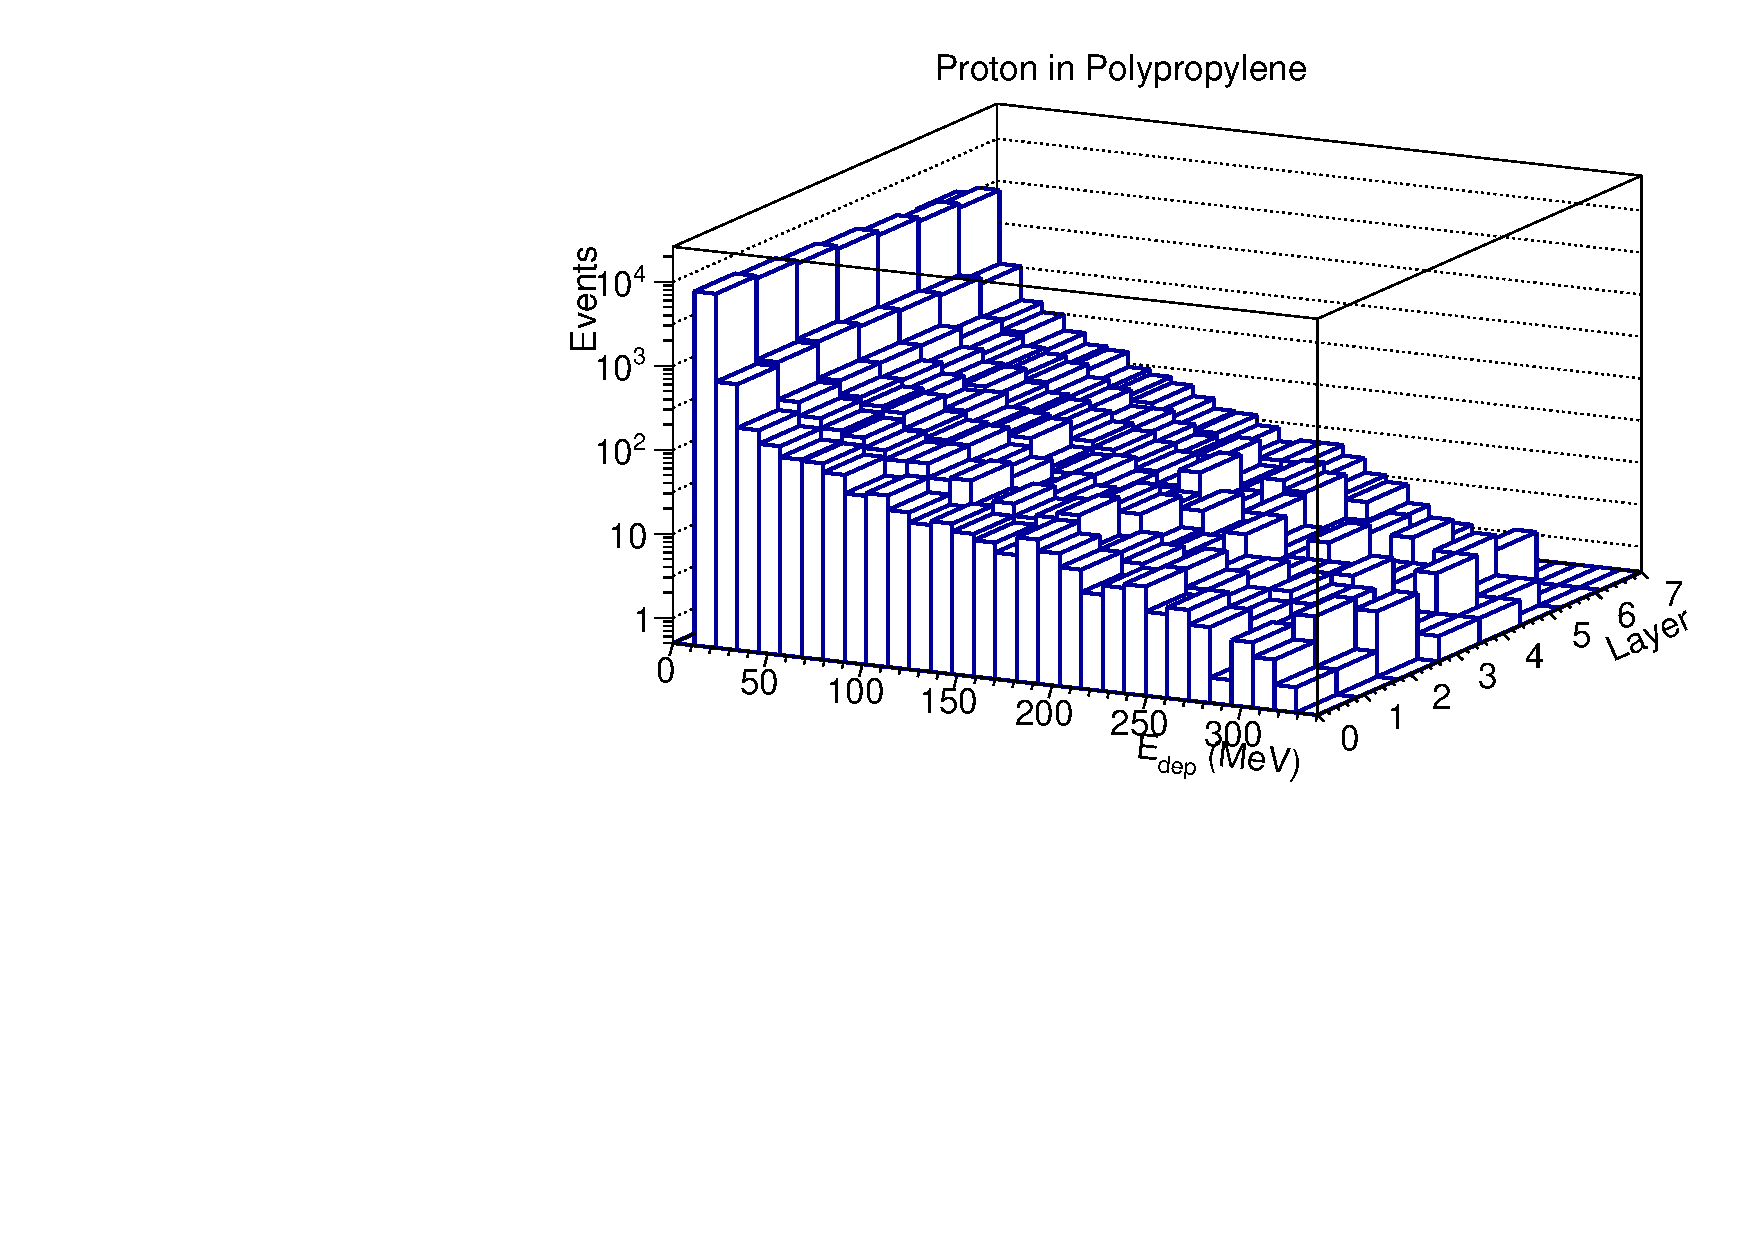
\includegraphics[width=.45\textwidth]{plots/P_pp_edep.pdf}
  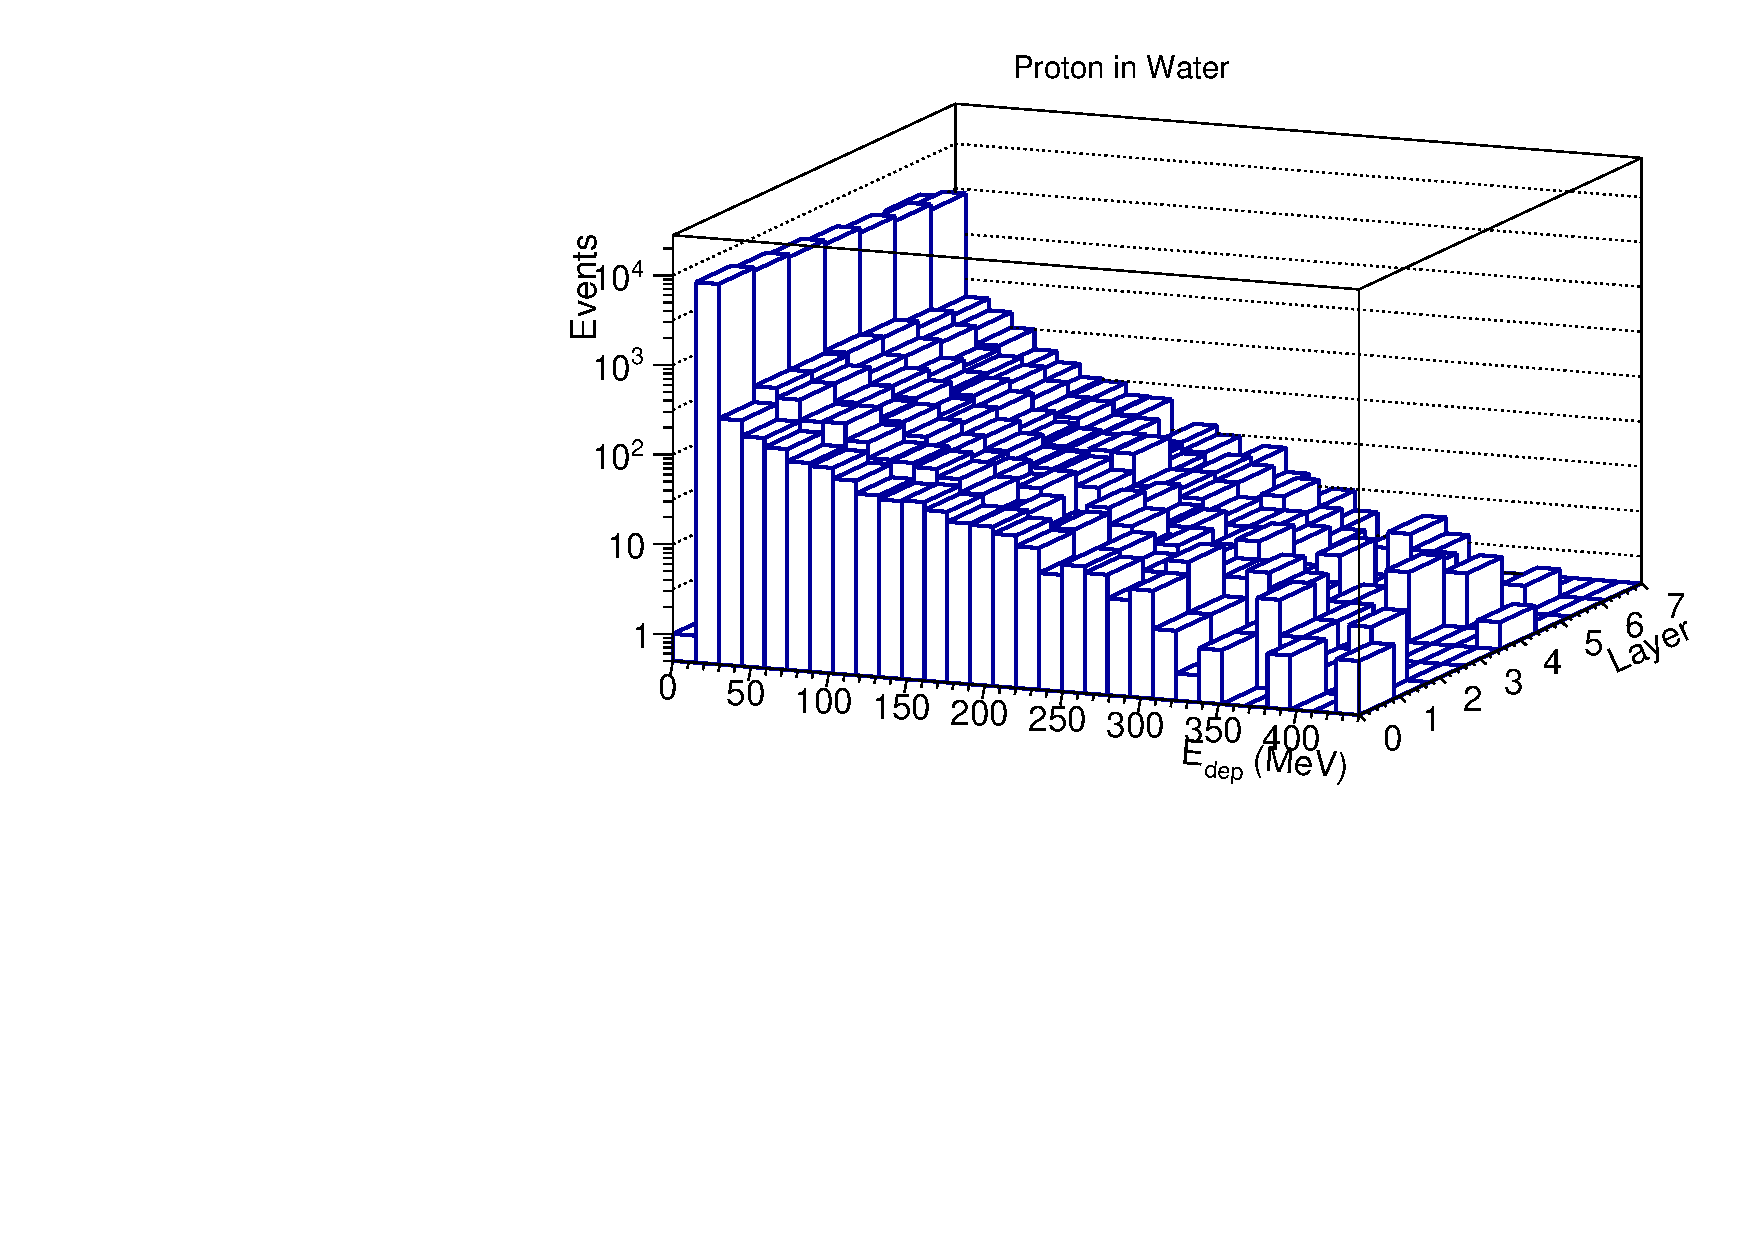
\includegraphics[width=.45\textwidth]{plots/P_h2o_edep.pdf}
  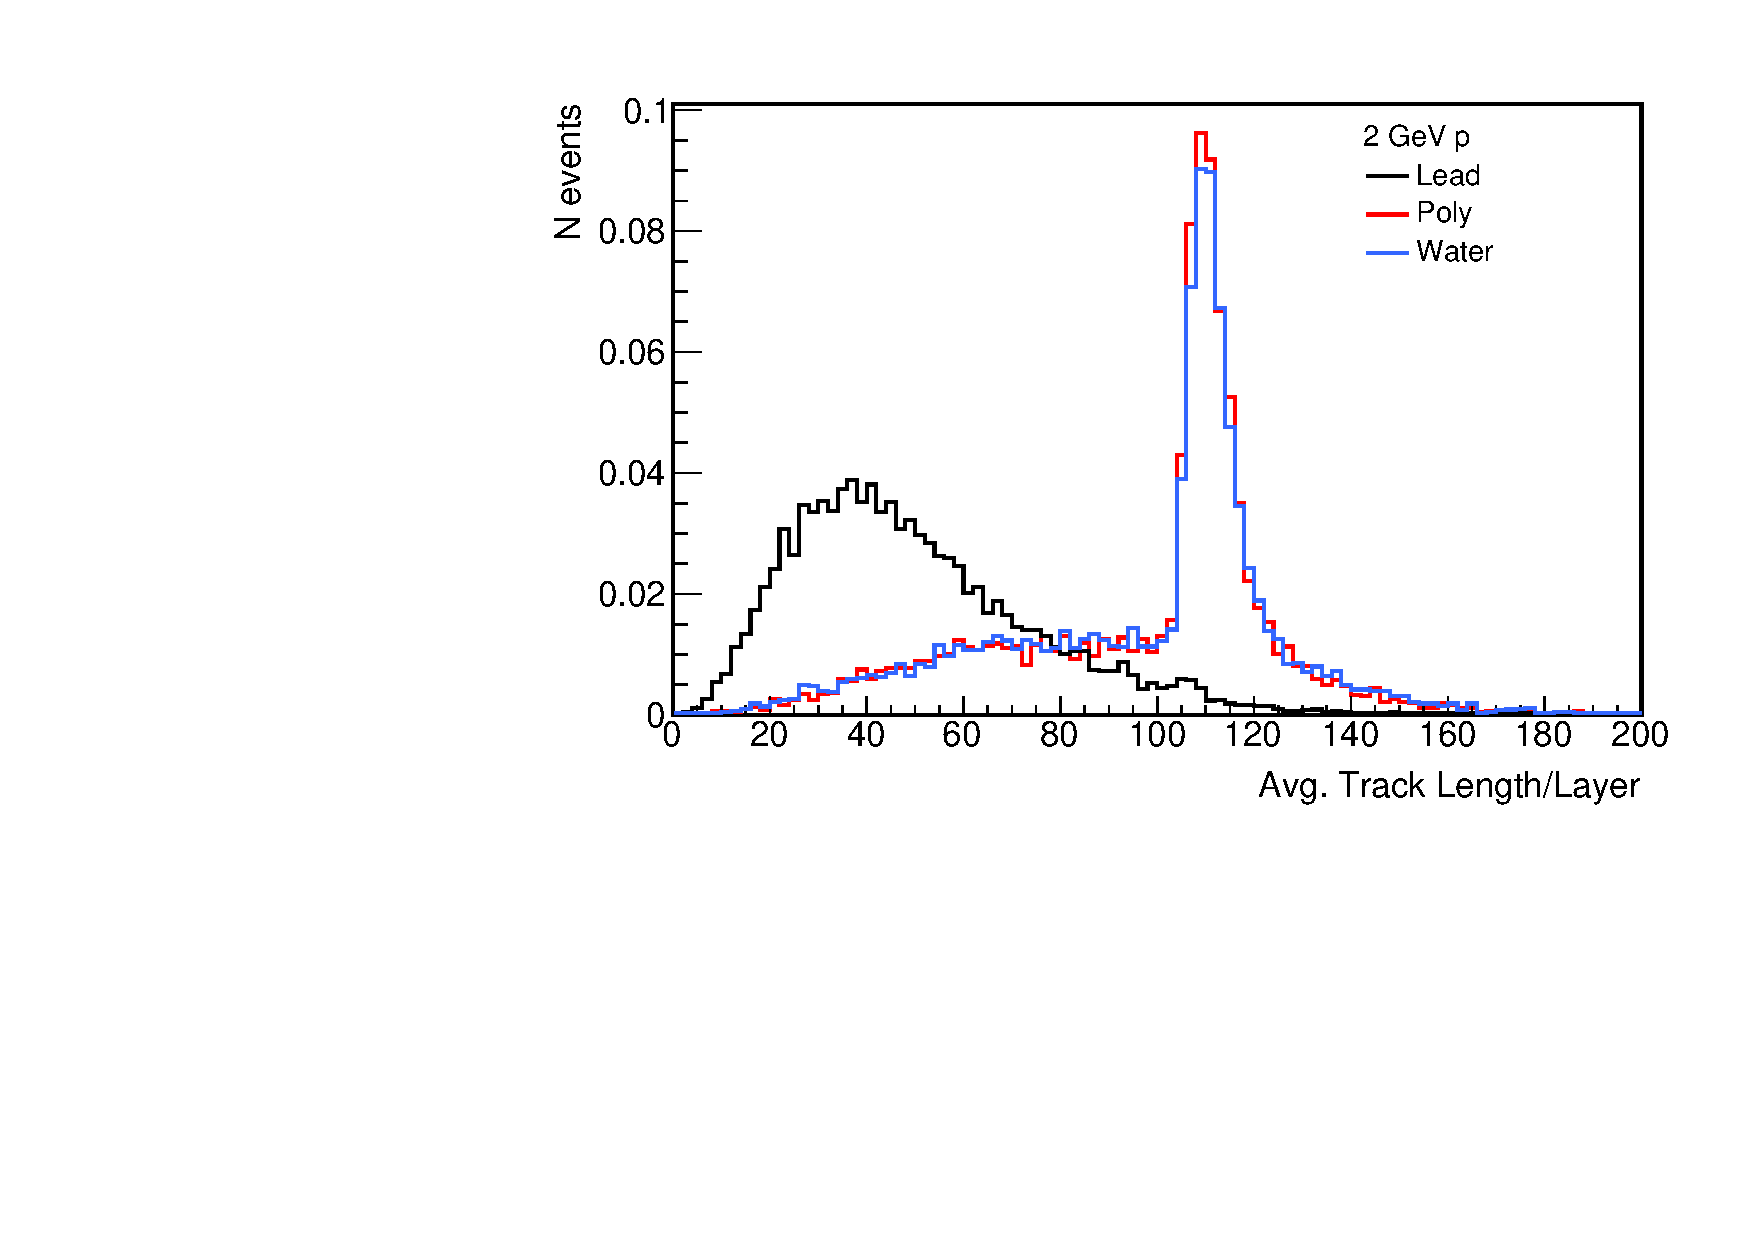
\includegraphics[width=.45\textwidth]{plots/TL_proton.pdf}
  \caption{Proton Plots, Pb $E_{\text{dep}}$ plot effectively has units of GeV not MeV, the $10^3$ is obscured.}
  \label{fig:p-quant}
\end{figure*}

\begin{figure*}
  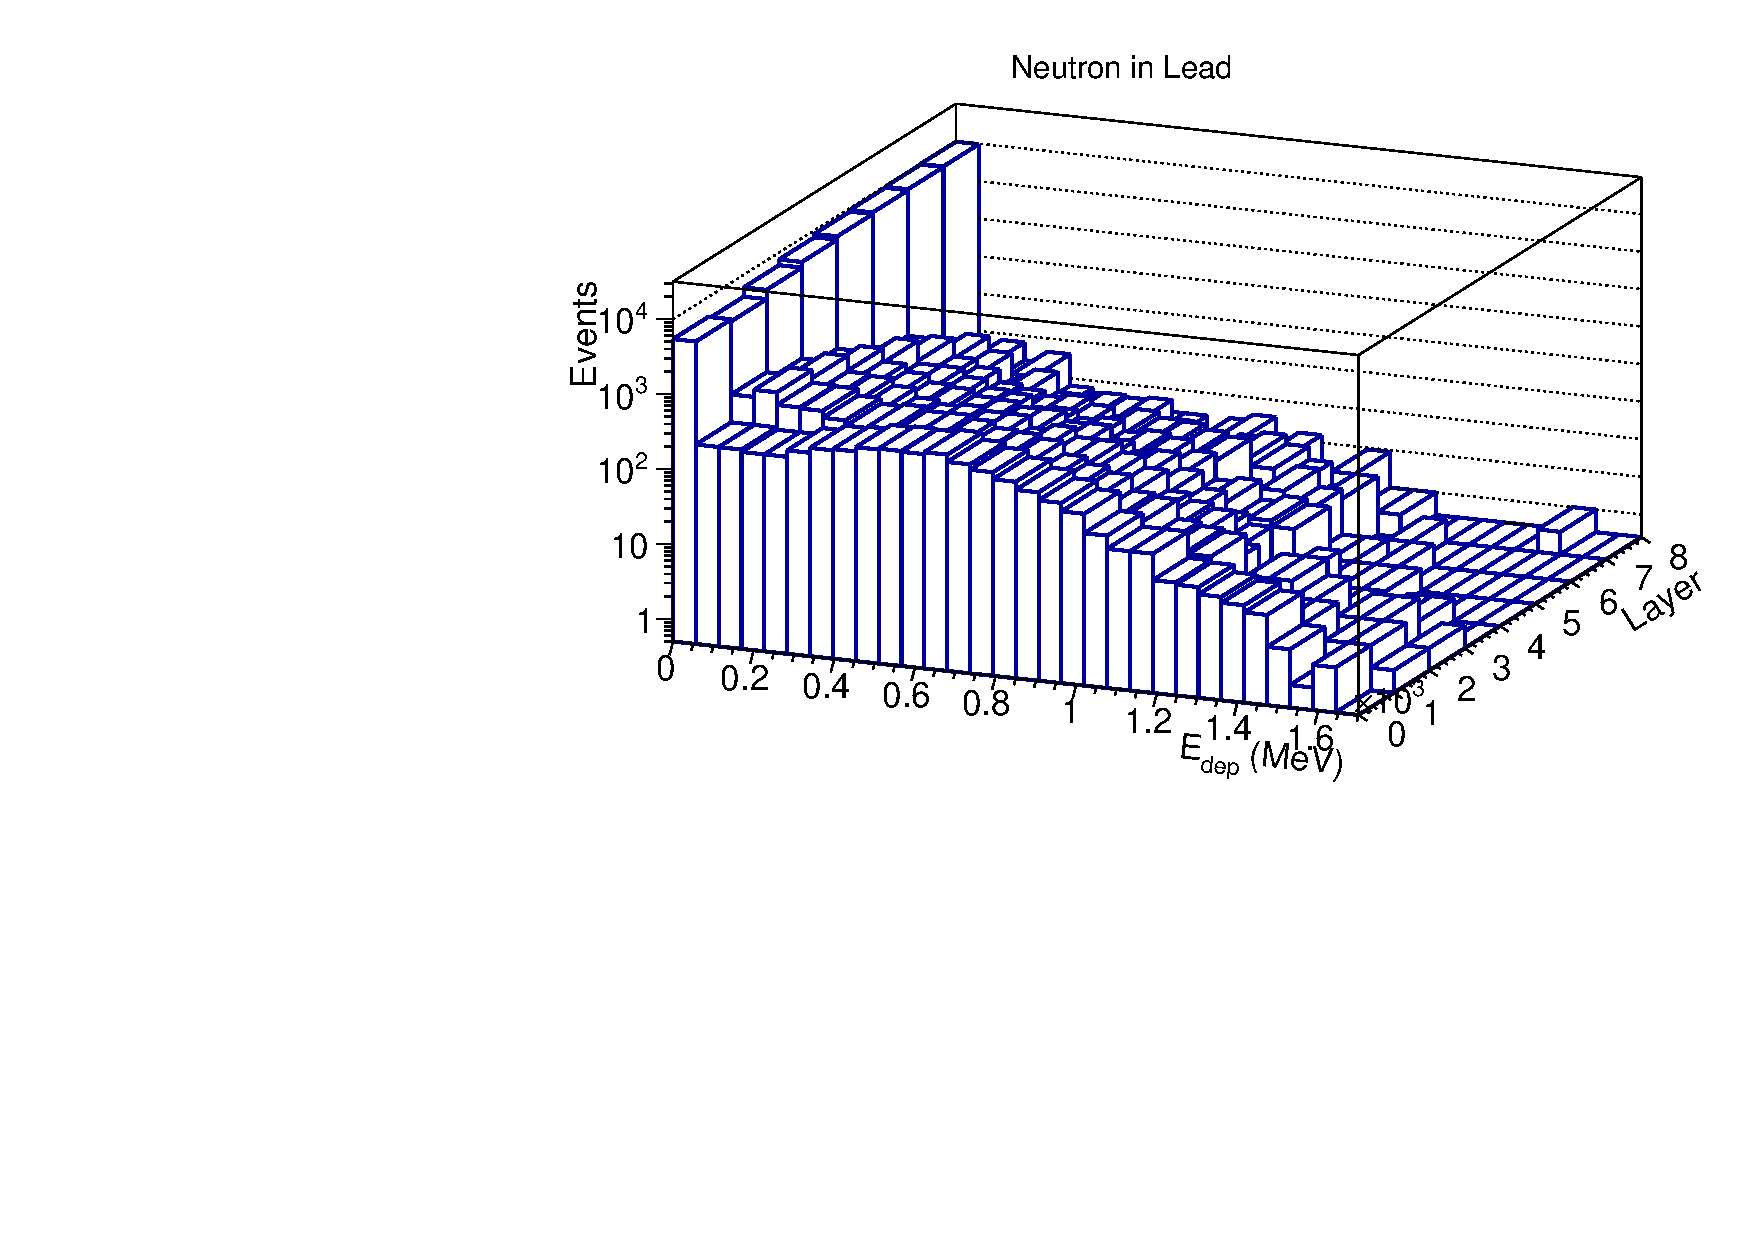
\includegraphics[width=.45\textwidth]{plots/N_pb_edep.pdf}
  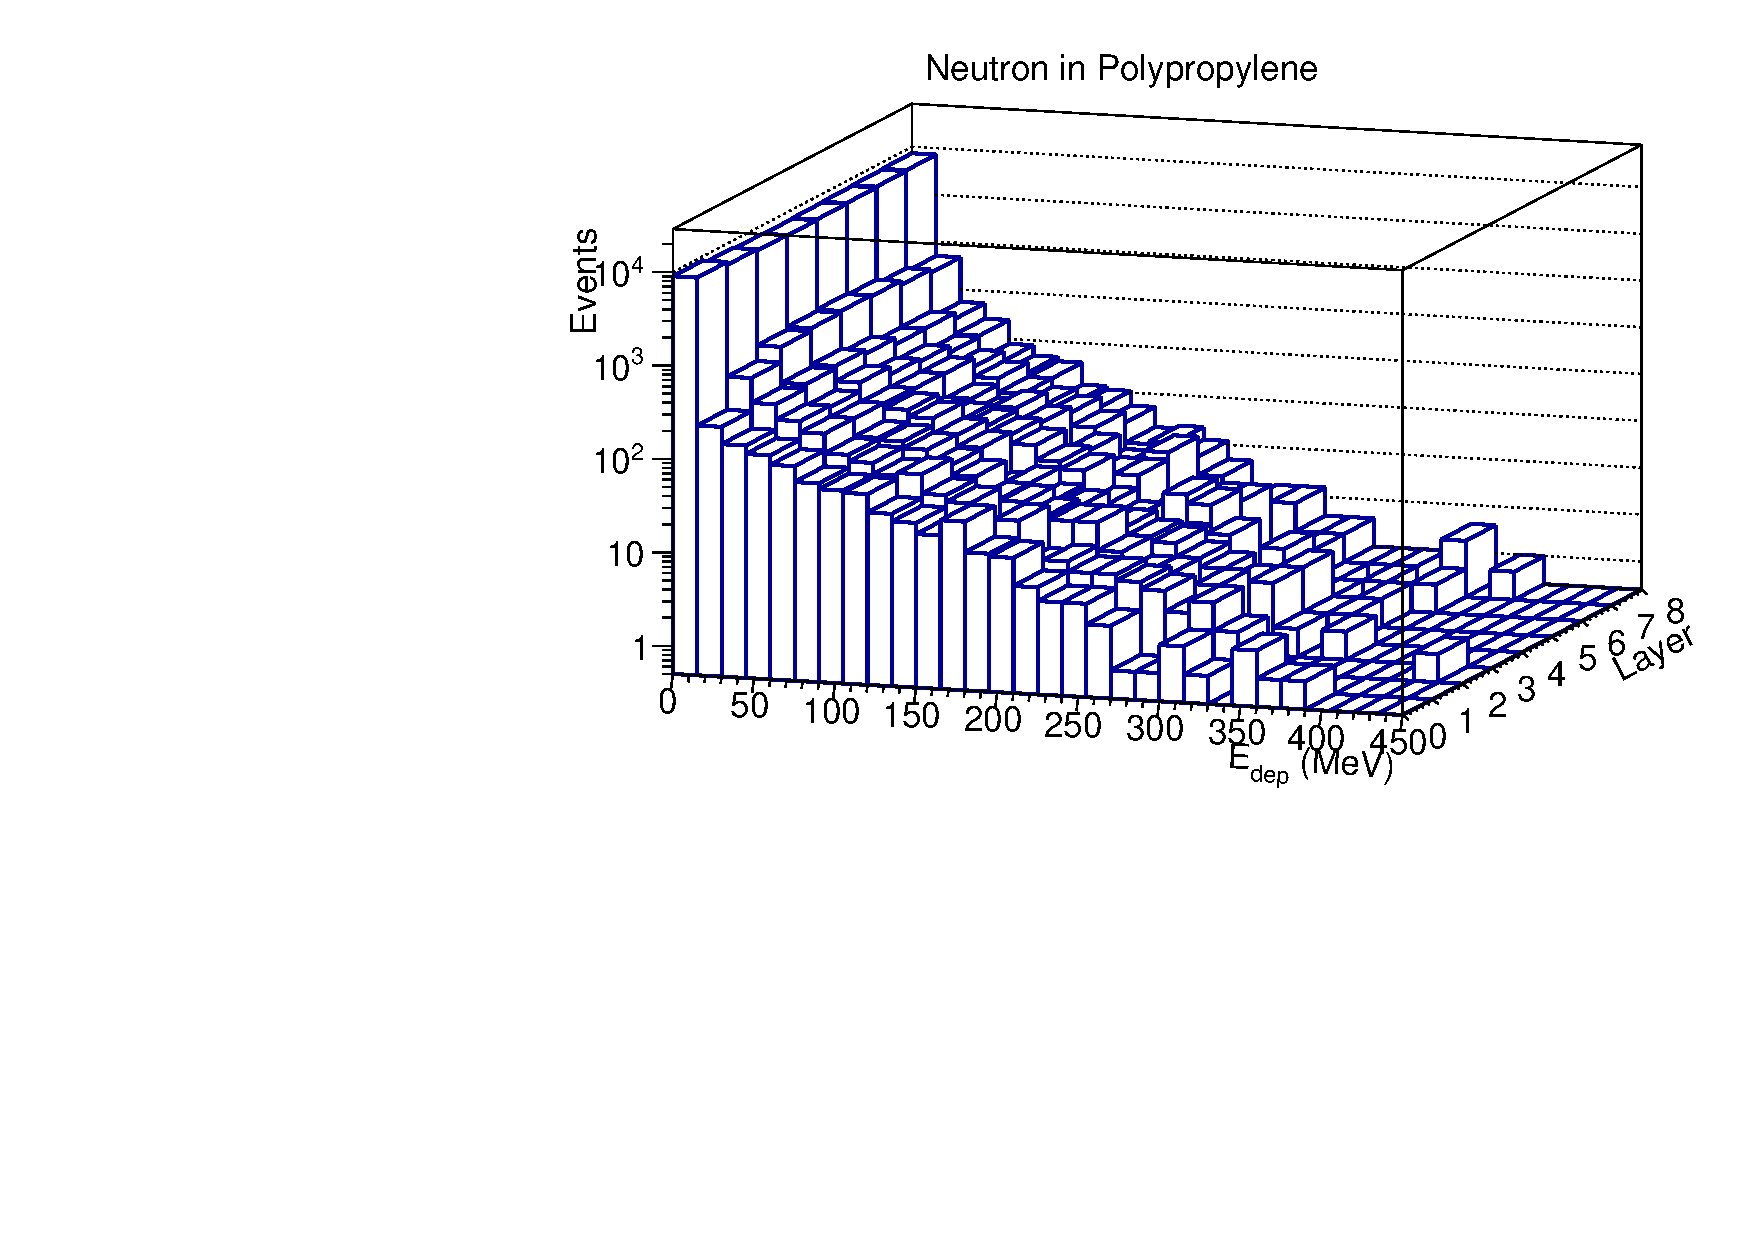
\includegraphics[width=.45\textwidth]{plots/N_pp_edep.pdf}
  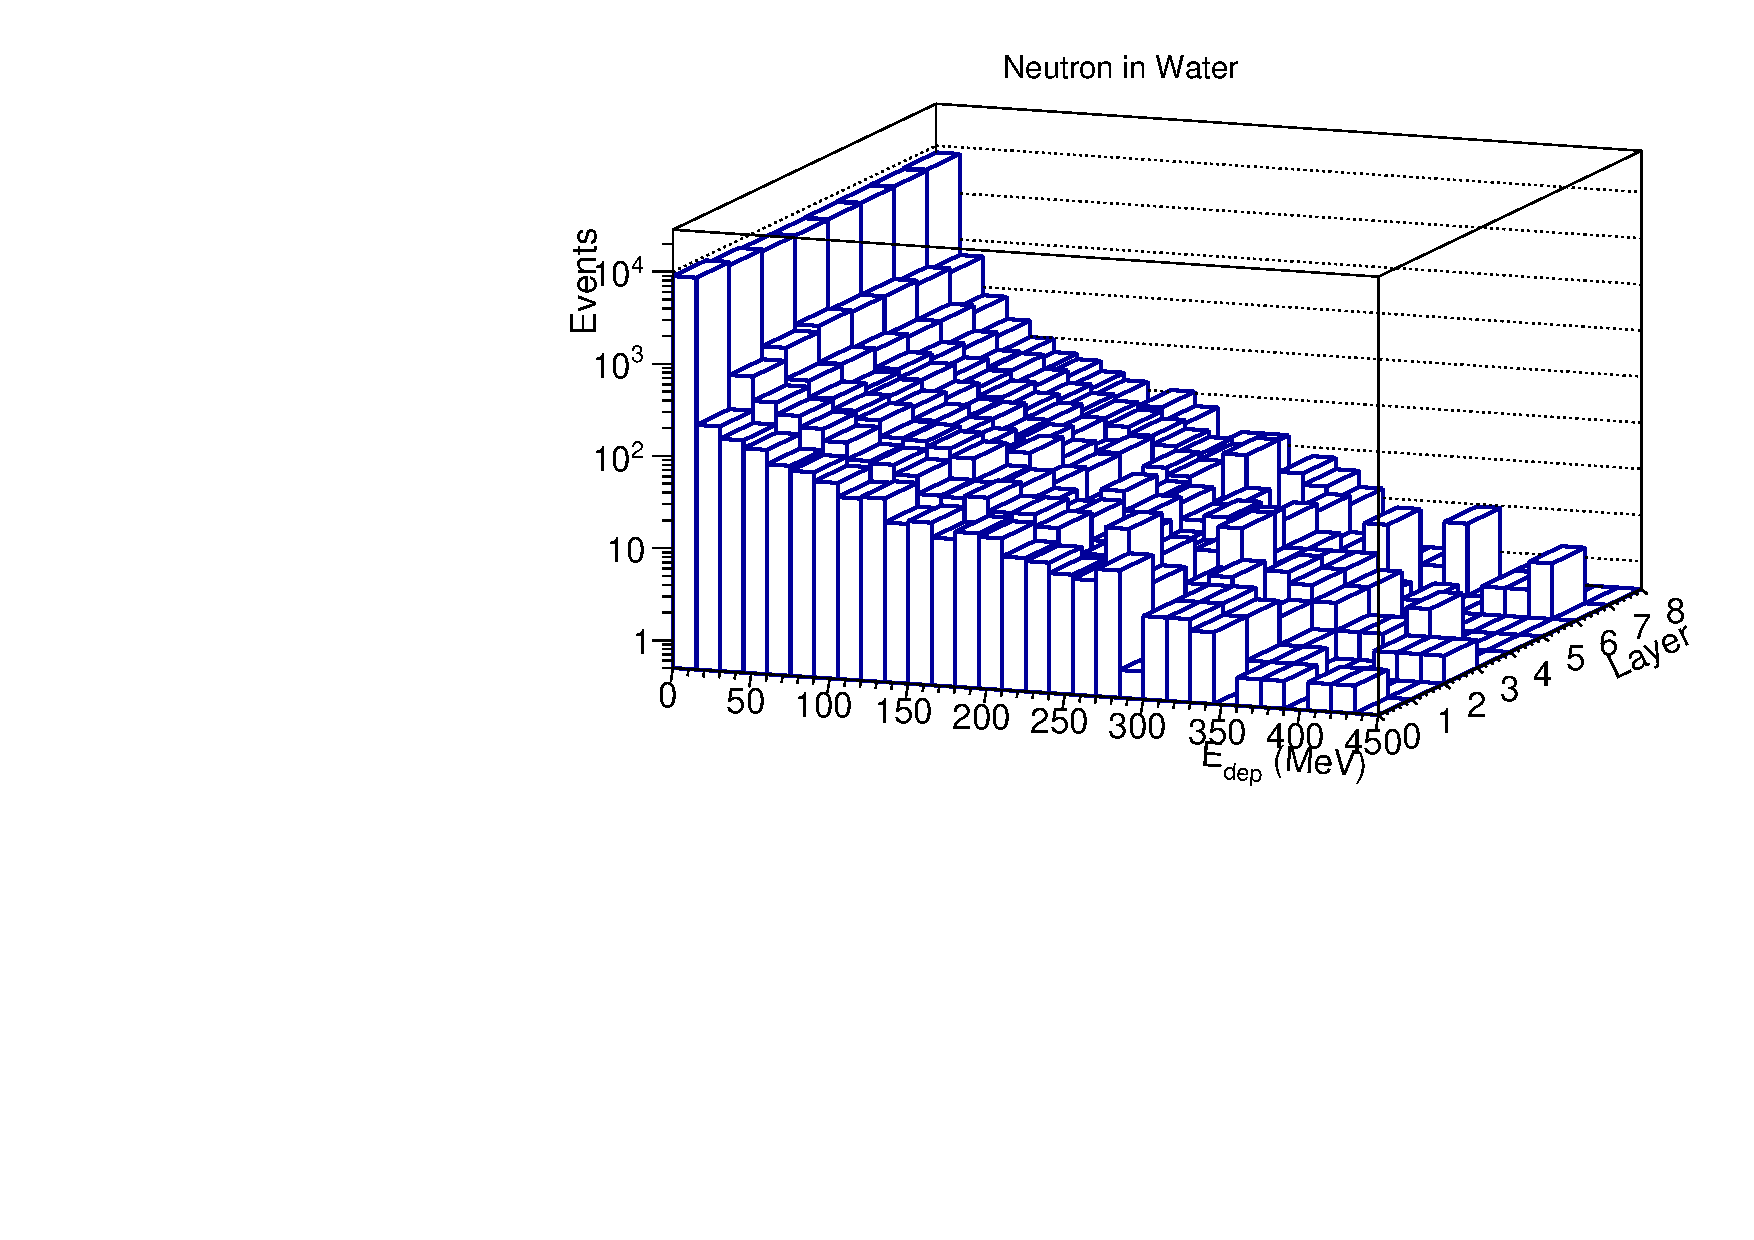
\includegraphics[width=.45\textwidth]{plots/N_h2o_edep.pdf}
  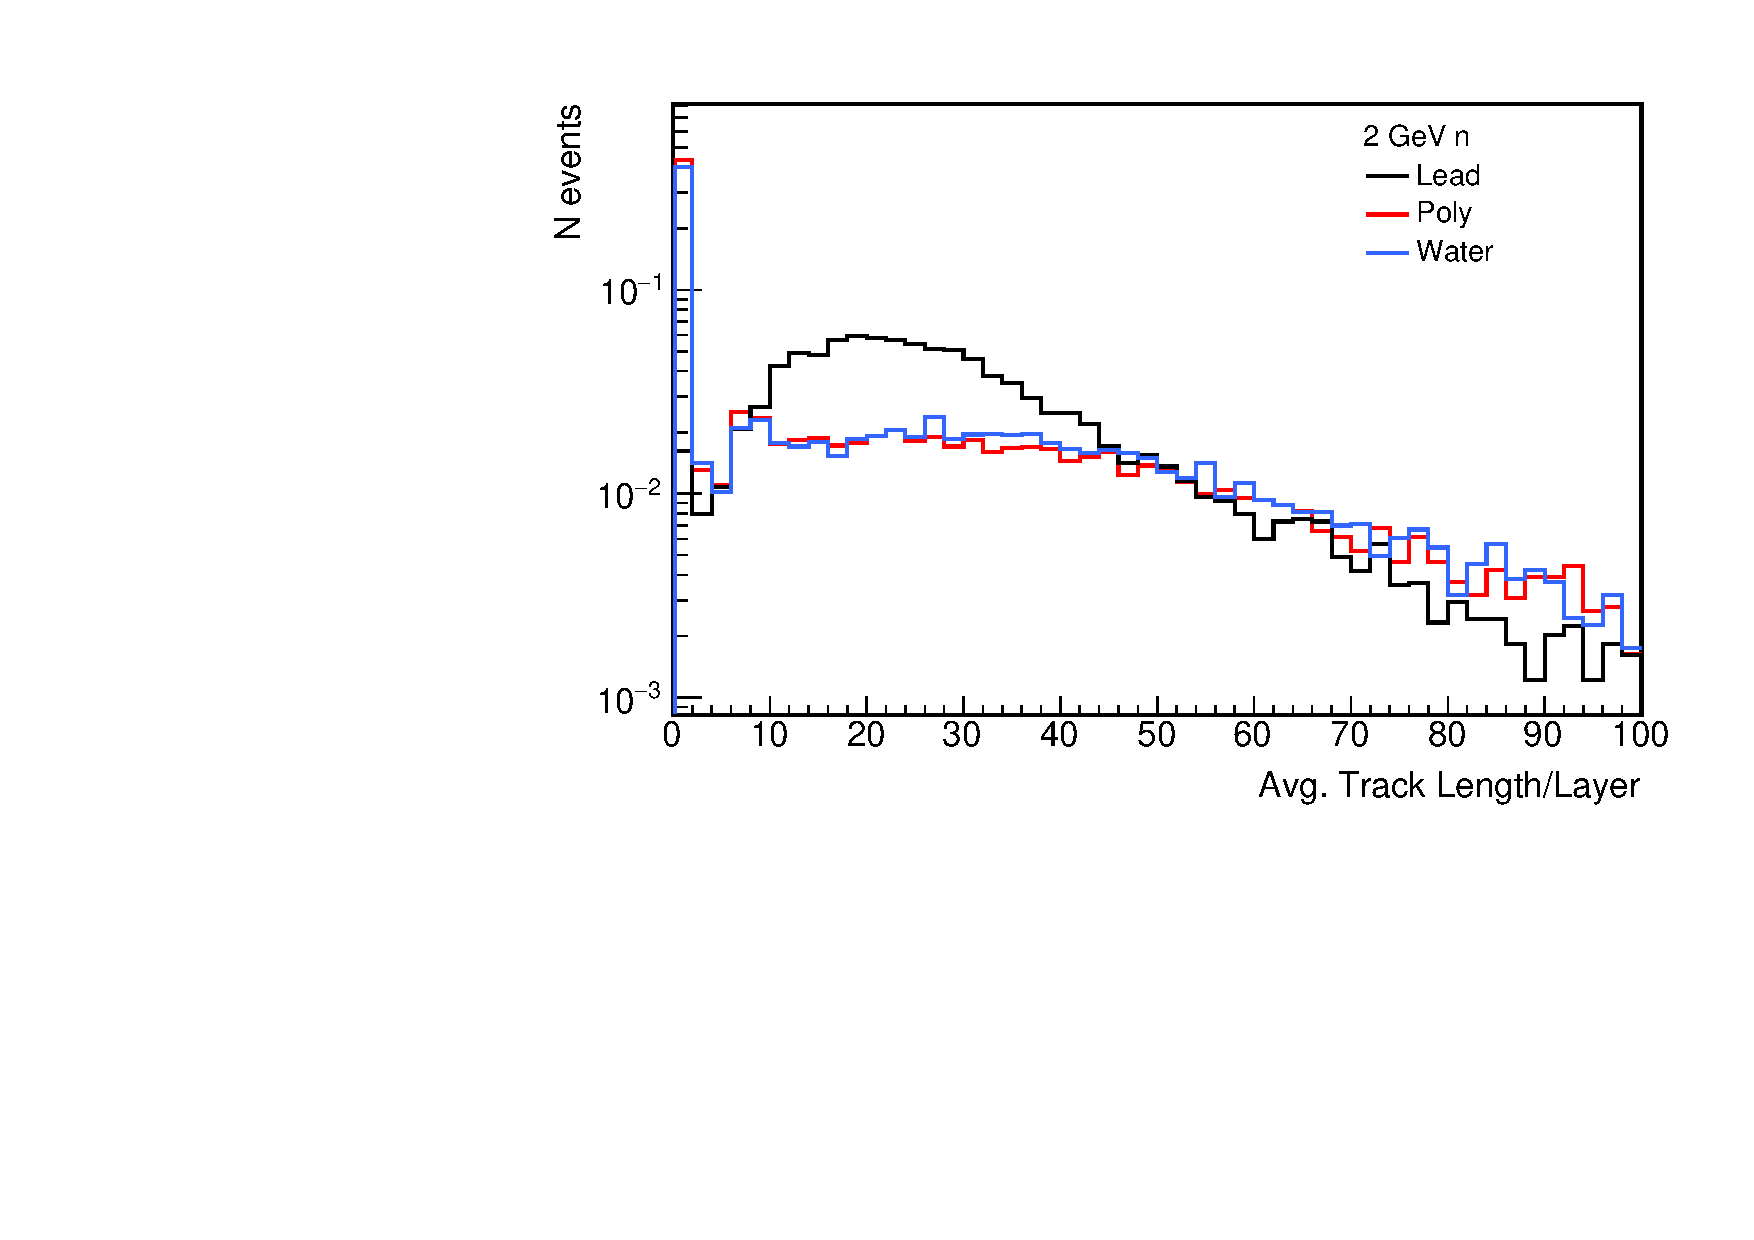
\includegraphics[width=.45\textwidth]{plots/TL_neutron.pdf}
  \caption{Neutron Plots, Pb $E_{\text{dep}}$ plot effectively has units of GeV not MeV, the $10^3$ is obscured.}
  \label{fig:n-quant}
\end{figure*}

\section{Conclusions}
This report introduced the very powerful, \texttt{C++} based  Geant4 software package for the simulation of the passage of particles through matter. We discussed the minimum requirements for a working Geant4 simulation, and also described some optional features of Geant4. We discussed our development of a simple system which was born from a Geant4 collaboration provided example. Some quantitative results were shown and discussed, and some qualitative discussion was presented. Some expected distributions were observed, while event displays showed some expected results as well. The code for this project can be found here:\\ \url{http://github.com/dougphy/p1_505}.

\begin{thebibliography}{9}
\bibitem{geant}
  GEANT4 Collaboration, S. Agostinelli et al., \textit{GEANT4: A Simulation toolkit}, Nucl. Instr. Meth. \textbf{A506} (2003) 250.
\bibitem{G4_tutorials}
  GEANT4 Collaboration, S. Agostinelli et al., \url{http://geant4.web.cern.ch/geant4/UserDocumentation/Doxygen/examples_doc/html/index.html}
\bibitem{ROOT}
  R.~Brun and F.~Rademakers, Nucl.\ Instrum.\ Meth.\ A {\bf 389}, 81 (1997). \texttt{http://root.cern.ch/}
\end{thebibliography}

\begin{appendix}

\section{Volumes in Detector Construction}\label{sec:AppendixA}
There are three definitions of volumes that need to be understood in detector construction. The ``world volume'' is the volume in which everything exists. The user defines the shape and properties of the world volume and then everything of interest, including any physical objects or shot particles, must be contained inside the world volume. If a particle track takes it outside the world volume, it is no longer considered part of the simulation. A ``logical volume'' has a physical shape and characteristics such as material and dimensions. This might be a block of NaI or a sphere of air. A ``physical volume'' is an instance of a logical volume. This volume is given coordinates within the world volume. The user may make one or more copies of a logical volume within the world volume (meaning one or more physical volumes). These are the actual blocks of matter in which the simulation will occur.
\section{Run and Event Actions}\label{sec:AppendixB}
The \texttt{RunAction} class in Geant4 gives the user the ability to control what happens at the beginning of an event and at the end of an event. Other member functions can be added to the class to give the user more control of what happens during a run. What is defined in the \texttt{RunAction} cannot be changed on an event by event basis. The \texttt{EventAction} class is similar to \texttt{RunAction} but of course for an event. The user has control of what happens at the beginning of an event and at the end -- and also can add member functions for specific tasks to run during the events. For example, the user can define control statements so different things can happen for a given number of particles, or track length, or amount of energy deposited, etc. in an event.

\end{appendix}

\end{document}
